\documentclass[12pt,a4paper]{article}

\usepackage{xeCJK}
\usepackage{amsmath}
\usepackage{hyperref}
\usepackage{amsfonts}
\usepackage{amssymb}
\usepackage{graphicx}
\usepackage{tikz}
\usepackage{pgf}
\usepackage{enumitem}
\renewcommand{\contentsname}{目\hspace{2em}录}
\renewcommand{\figurename}{图}
\renewcommand{\tablename}{表}
% \renewcommand{\partname}{部分}
\renewcommand{\listfigurename}{插图目录}
\renewcommand{\listtablename}{表格目录}
\renewcommand{\refname}{参考文献}
\renewcommand{\appendixname}{附录}
\renewcommand{\indexname}{索\hspace{2em}引}
\renewcommand{\theequation}{\arabic{section}.\arabic{equation}}
\title{机器学习笔记}
\author{邹智鹏}
\begin{document}
  \maketitle
  \tableofcontents
  \newpage
  \section{特征分解}
  对于$m\times m$矩阵$\mathbf{A}$,特征分解可定义为:$\mathbf{A}\mathbf{x}=\lambda \mathbf{x}$. 其中,$\lambda$为特征值,$\mathbf{x}$为特征值所对应的特征向量。

  \textbf{例:} 对矩阵$\left(\begin{array}{ccc}
    1 & 1 & 0 \\ 
    1 & 2 & 1 \\ 
    0 & 1 & 1 \\ 
  \end{array}\right)$进行特征分解,并求特征值及特征向量。

  \textbf{解:} 根据定义,则有$\mathbf{Ax} = \lambda \mathbf{x} \Rightarrow \left(\mathbf{A} - \lambda \mathbf{E}\right)\mathbf{x}=0$
  
  由于$\mathbf{x}$行列式不为0,则有$\left|\mathbf{A}-\lambda \mathbf{E}\right|=0$,即
  $$
    \left|\left(\begin{array}{ccc}
      1-\lambda & 1 & 0 \\ 
      1 & 2 - \lambda & 1 \\ 
      0 & 1 & 1 - \lambda 
    \end{array}\right)\right| = 0
  $$
  根据行列式计算规则\footnote{行列式计算,需取不同行不同列的元素相乘,再带上$(-1)^{i+j}$作为符号,$i, j$为行与列索引。},则有
  $$
  \begin{aligned}
    & (1-\lambda)(2-\lambda)(1-\lambda) - 2(1-\lambda) = 0 \\ 
    & (1-\lambda)((2-\lambda)(1-\lambda)-2) = 0
  \end{aligned}
  $$
  根据上式可得$\lambda _1 = 1$. 则有
  $$
   \begin{aligned}
    & (2-\lambda)(1-\lambda)-2 = 0 \\ 
    & \lambda ^2 -3\lambda +2 - 2 = 0 \\ 
    & \lambda _2 = 0, \lambda _3 = 3
   \end{aligned}
  $$
  将$\mathbf{\lambda}$代入$\mathbf{A} - \lambda \mathbf{E}=0$,则当$\lambda _1 = 1$时,有 
  $$
  \left(\begin{array}{ccc}
    0 & 1 & 0 \\ 
    1 & 1 & 1 \\ 
    0 & 1 & 0 \\ 
  \end{array}\right)\times \left(\begin{array}{c}
    x_1 \\ 
    x _2 \\ 
    x _3 
  \end{array}\right) = 0
  $$
  则可列出方程组 
  $$
  \left\{\begin{array}{l}
    0\cdot x_1 + 1 \cdot x_2 + 0 \cdot x_3 = 0 \\ 
    x_1 + x_2 + x_3 = 0 \\ 
    x_2 = 0
  \end{array}\right. \Rightarrow x_1 + x_3 = 0
  $$
  则可得出基础解系$\mathbf{x} = \left(\begin{array}{c}
    1 \\ 
    0 \\ 
    -1
  \end{array}\right)$,令 $||\mathbf{x}||_2=1$,则$x^2+x^2=1 \Rightarrow x = \frac{1}{\sqrt{2}}$.
  同理,当$\lambda _2 = 0$时,有 
  $$
  \left\{\begin{array}{l}
    x_1 + x_2 = 0 \\ 
    x_1 + 2x_2+x_3 = 0 \\ 
    x_2 + x_3 = 0
  \end{array}\right. \Rightarrow \mathbf{x} = \left(\begin{array}{c}
    1 \\ 
    -1 \\ 
    1
  \end{array}\right) \Rightarrow \mathbf{x} = \left(\begin{array}{c}
    \frac{1}{\sqrt{3}} \\ 
    -\frac{1}{\sqrt{3}} \\ 
    \frac{1}{\sqrt{3}}
  \end{array}\right)
  $$
  当$\lambda _3 = 3$时,有 
  $$
  \left\{\begin{array}{c}
    -2x_1 + x_2 = 0 \\ 
    x_1 - x_2 +x_3 = 0 \\ 
    x_2 -2x_3 = 0
  \end{array}\right. \Rightarrow \mathbf{x} = \left(\begin{array}{c}
    1 \\ 
    2 \\ 
    1
  \end{array}\right) \Rightarrow \mathbf{x} = \left(\begin{array}{c}
    \frac{1}{\sqrt{6}} \\ 
    \frac{2}{\sqrt{6}} \\ 
    \frac{1}{\sqrt{6}}
  \end{array}\right)
  $$
  \section{SVD分解}
  矩阵的特征分解,只能适用于当矩阵$\mathbf{A}$为方阵的情况,但对于多数矩阵而言,其并不为方阵,如$\mathbf{A} \in \mathbb{R}^{m\times n}$,对其分解便是奇异值分解。我们定义,SVD分解采用如下表达式进行:
  \begin{equation}
    \mathbf{A} = \mathbf{UD}\mathbf{V}^{\top}
  \end{equation}
  其中,$\mathbf{U}$的列向量,称为$\mathbf{A}$的左奇异值向量,而$\mathbf{V}$的列向量则称为$\mathbf{A}$的右奇异值向量。若$\mathbf{A} \in \mathbb{R}^{m\times n}$,则$\mathbf{U} \in \mathbb{R}^{m \times m}, \mathbf{V} \in \mathbb{R}^{n \times n}$,$\mathbf{D}$为奇异值矩阵,对角线为奇异值。实际上,在求解过程中,$\mathbf{A}$的左奇异值向量为$\mathbf{AA}^{\top}$的特征向量,$\mathbf{A}$的右奇异值向量为$\mathbf{A}^{\top}\mathbf{A}$的特征向量。而$\mathbf{A}$的非零奇异值为$\mathbf{AA}^{\top}$特征值的平方根,同时也是$\mathbf{A}^{\top}\mathbf{A}$特征值的平方根。

  \textbf{例:} 对矩阵$\mathbf{A} = \left(\begin{array}{cc}
    0 & 1 \\ 
    1 & 1 \\ 
    1 & 0
  \end{array}\right)$
  进行SVD分解。

  \textbf{解:} 分别求得左奇异值向量的基础矩阵$\mathbf{U'} = \mathbf{AA}^{\top}$与右奇异值矩阵的基础矩阵$\mathbf{V'} = \mathbf{A}^{\top}\mathbf{A}$。
  $$
  \mathbf{U'} = \left(\begin{array}{ccc}
    1 & 1 & 0 \\ 
    1 & 2 & 1 \\ 
    0 & 1 & 1
  \end{array}\right)
  $$
  对其进行特征分解,可得特征值$\lambda _1 = 1, \lambda _2 = 0, \lambda _3 = 3$. 对应特征向量为$u_1 = \left(\begin{array}{c}
    \frac{1}{\sqrt{2}} \\ 
    0 \\ 
    -\frac{1}{\sqrt{2}}
  \end{array}\right), u_2 = \left(\begin{array}{c}
    \frac{1}{\sqrt{3}} \\ 
    -\frac{1}{\sqrt{3}} \\ 
    \frac{1}{\sqrt{3}}
  \end{array}\right), u_3 = \left(\begin{array}{c}
    \frac{1}{\sqrt{6}} \\ 
    \frac{2}{\sqrt{6}} \\ 
    \frac{1}{\sqrt{6}}
  \end{array}\right)$
  由$\mathbf{A}^{\top}\mathbf{A}$可得
  $$
  \mathbf{V'} = \left(\begin{array}{cc}
    2 & 1 \\ 
    1 & 2 \\ 
  \end{array}\right)
  $$
  对其进行特征分解,可得特征值$\lambda _1 = 1, \lambda _2 = 3$. 对应得特征向量为
  $v_1 = \left(\begin{array}{c}
    -\frac{1}{\sqrt{2}} \\ 
    \frac{1}{\sqrt{2}}
  \end{array}\right), v_2 = \left(\begin{array}{c}
    \frac{1}{\sqrt{2}} \\ 
    \frac{1}{\sqrt{2}} 
  \end{array}\right)$. 根据特征值及特征向量,可得奇异值,计算方式为$\mathbf{A}v_i=\sigma u_i$,其中$v_i$为$\mathbf{A}^{\top}\mathbf{A}$的特征向量,$u_i$为$\mathbf{AA}^\top$的特征向量。 

  当$\lambda _1 = 1, u_1, v_1$时,有
  $$
  \left(\begin{array}{cc}
    0 & 1 \\ 
    1 & 1 \\ 
    1 & 0
  \end{array}\right) \times \left(\begin{array}{c}
    -\frac{1}{\sqrt{2}} \\ 
    \frac{1}{\sqrt{2}}
  \end{array}\right) = \sigma \left(\begin{array}{c}
    \frac{1}{\sqrt{2}} \\ 
    0 \\ 
    -\frac{1}{\sqrt{2}}
  \end{array}\right)
  $$
  解得,$\sigma = 1$. 同理,可得$\sigma _2 = \sqrt{3}$\footnote{可根据特征值的平方根求得对应的奇异值$\sigma$.}.
  \section{PCA主成分分析}

  PCA是一种数据降维的有效方法,其在于将高维度的数据转换为低纬度的空间中。直观地解释便是,在二维空间中,有点$(x,y)$,若选取不同的坐标系,则点的表示将会发生改变。如将原有的坐标系进行旋转,使其能够更好地区分数据(方差较大)但却保有最近重构性(点离坐标的距离够近)。因此PCA分析方法有两个原则:
  \begin{enumerate}
    \item 最近重构性:样本点到超平面的距离足够近;
    \item 最大可分画性:样本点在超平面上的投影能尽可能地分开。
  \end{enumerate}

  从概念上分析,可知PCA分析实际上是进行一系列的基变换(相当于坐标轴变换)。所谓的坐标轴旋转,即是对已有的坐标,按照正交基在一定的方向上进行变换,从而改变数据的表示。因此从本质上将,PCA分析实际上是矩阵相乘所得的矩阵变换。该特征通过最优化推导,也可推出。

  设对于向量$\mathbf{x}$其存在一个编码函数使得$\mathbf{c}=g(\mathbf{x})=\mathbf{Dx}$,同时存在一个解码函数为$f(x)$使得$\mathbf{x}=f(\textbf{c})$. 设$\mathbf{x}$对应的最优编码为$\mathbf{c}^*$,则最优编码函数$g(x)$应使得误差最小,即
  $$
  \mathbf{c}^* = \arg\min\limits_{\mathbf{c}} \Arrowvert \mathbf{x}-f(\mathbf{c}) \Arrowvert _2^2
  $$
  由于$\mathbf{x}$与$f(\mathbf{c})$为一个向量,则上式为
  $$
  \mathbf{c}^* = \arg\min\limits_{\mathbf{c}} \left((\mathbf{x}-f(\mathbf{c}))^\top(\mathbf{x}-f(\mathbf{c}))\right)
  $$
  对$(\mathbf{x}-f(\mathbf{c}))^\top(\mathbf{x}-f(\mathbf{c}))$进行化简,可得
  $$
  \begin{aligned}
    &\mathbf{x}^\top \mathbf{x} - \mathbf{x}^\top f(\mathbf{c}) - f(\mathbf{c})^\top \mathbf{x} + f(\mathbf{c})^\top f(\mathbf{c}) \\ 
    =& \mathbf{x}^\top \mathbf{x} - 2\mathbf{x}^\top f(\mathbf{c}) + f(\mathbf{c})^\top f(\mathbf{c})\\
    =& \mathbf{x}^\top \mathbf{x} -2\mathbf{x}^\top \mathbf{Dc}+(\mathbf{Dc})^\top \mathbf{Dc}
  \end{aligned}
  $$

  此外,根据PCA分析的原理,对于主成分分析,实际上是对数据进行矩阵变换,即对于一个矩阵$\mathbf{P}=\left[\begin{array}{c}
    \mathbf{p}_1 \\ 
    \mathbf{p}_2 \\ 
    \vdots \\ 
    \mathbf{p}_R
  \end{array}\right]$,对于原始数据矩阵$\mathbf{X}=\left[\begin{array}{cccc}
    \mathbf{x}_1, \mathbf{x}_2, \cdots, \mathbf{x}_M
  \end{array}\right]$
  其中,$\mathbf{p}_i$为行向量,即$\mathbf{p}_i \in \mathbb{R}^{1*N}$,$\mathbf{x}_i$为列向量,即$\mathbf{x}_i \in \mathbb{R}^{N*1}$,则
  $$
  \mathbf{P}\times \mathbf{X} = \left[\begin{array}{c}
    \mathbf{p}_1 \\ 
    \mathbf{p}_2 \\ 
    \vdots \\ 
    \mathbf{p}_R
  \end{array}\right] \times \left[\begin{array}{cccc}
    \mathbf{x}_1, \mathbf{x}_2, \cdots, \mathbf{x}_M
  \end{array}\right] = \left[\begin{array}{cccc}
    \mathbf{p}_1\mathbf{x}_1 & \mathbf{p}_1\mathbf{x}_2 & \cdots & \mathbf{p}_1\mathbf{x}_M \\ 
    \mathbf{p}_2\mathbf{x}_1 & \mathbf{p}_2\mathbf{x}_2 & \cdots & \mathbf{p}_2\mathbf{x}_M \\ 
    \vdots & \cdots & \ddots & \vdots \\ 
    \mathbf{p}_R\mathbf{x}_1 & \mathbf{p}_R\mathbf{x}_2 & \cdots & \mathbf{p}_R\mathbf{x}_M \\ 
  \end{array}\right]
  $$
  即$\mathbf{P}\times \mathbf{X} \in \mathbb{R}^{R*M}$,对于原始矩阵$\mathbf{X} \in \mathbb{R}^{N\times M}$,若$R < N$,则说明最终变换结果的维度小于变换前的维度,从而实现了降维。

  \textbf{上述变换同时说明,矩阵乘法的意义在于将矩阵乘右侧的列向量映射变换到左侧行向量所表示的方向和空间中去}。

  根据最大可分性原则,需要保证在经过变换后,样本点在超平面的投影的方差足够大。其中方差可表示为:
  $$
  Var(\mathbf{X})= \frac{1}{m} \sum\limits_{i=1}^m \left(x_i-\mu\right)^2
  $$
  其中$x_i$表示在经过降维后新的第$i$个数据样本的表示。由于在操作中我们会对样本进行中心化,即使其均值为0,则$Var(\mathbf{X})=\frac{1}{n}\sum\limits_{i=1}^m x_i^2$. 通常当到达该步时,便可通过最优化问题求解方法,找出使得方差最大的基从而得出结果,然而上述目标函数并不能直接使用作为求解方案(偏导数无法获得)。

  可以考虑更多的约束条件,如使用协方差保证在选取基时应当保证数据变换后不完全独立,即以协方差为0为优化目标。

  可以考虑,对于一个矩阵$\mathbf{X}$令其于其转置相乘,可的协方差矩阵,即$Cov(\mathbf{X}) = \mathbf{X} \mathbf{X}^\top$. 证明过程如下:

  设$\mathbf{X} = \left[\begin{array}{cccc}
    x^{(1)}_1 & x^{(1)}_2 & \cdots & x^{(1)}_m \\ 
    x^{(2)}_1 & x^{(2)}_2 & \cdots & x^{(2)}_m \\ 
    \vdots & \cdots & \ddots & \vdots \\ 
    x^{(n)}_1 & x^{(n)}_2 & \cdots & x^{(n)}_m \\ 
  \end{array}\right]$,则$\mathbf{X}^\top=\left[\begin{array}{cccc}
    x^{(1)}_1 & x^{(2)}_1 & \cdots & x^{(n)}_1 \\ 
    x^{(1)}_2 & x^{(2)}_2 & \cdots & x^{(n)}_2 \\ 
    \vdots & \cdots & \ddots & \vdots \\ 
    x^{(1)}_m & x^{(2)}_m & \cdots & x^{(n)}_m \\ 
  \end{array}\right]$,故$\mathbf{X} \times \mathbf{X}^\top$为
  $$
  \left[\begin{array}{cccc}
    \sum\limits_{i=1}^{m} \left(x_i^{(1)}\right)^2 & \sum\limits_{i=1}^{m} x_i^{(1)}x_i^{(2)} & \cdots &\sum\limits_{i=1}^{m} x_i^{(1)}x_i^{(n)} \\ 
    \sum\limits_{i=1}^{m} x_i^{(2)}x_i^{(1)} & \sum\limits_{i=1}^{n} \left(x_i^{(2)}\right)^2 & \cdots &\sum\limits_{i=1}^{n} x_i^{(2)}x_i^{(n)} \\ 
    \vdots & \cdots & \ddots & \vdots \\ 
    \sum\limits_{i=1}^{m} x_i^{(n)}x_i^{(1)} & \sum\limits_{i=1}^{m} x_i^{(n)}x_i^{(2)} & \cdots &\sum\limits_{i=1}^{m} \left(x_i^{(n)}\right)^2 \\ 
  \end{array}\right]
  $$
  协方差矩阵为对角矩阵,对角线为方差$Var(\mathbf{x}_m)$,其他为协方差。根据目标函数,需要将协方差优化为0,即将协方差矩阵转换为对角阵,则优化目标变为了协方差矩阵的对角化。

  设经过PCA变换后得到压缩后数据为$\mathbf{Y}$,即$\mathbf{Y}=\mathbf{P}\times \mathbf{X}$,其中$\mathbf{P},\mathbf{Y}$遵循上述定义。根据上述描述,设$\mathbf{C} = \mathbf{X} \mathbf{X}^\top$,为$\mathbf{X}$的协方差矩阵,而$\mathbf{D}=\mathbf{Y} \mathbf{Y}^\top$。

  $$
  \begin{aligned}
    \mathbf{D}=\mathbf{Y} \mathbf{Y}^\top = \mathbf{P} \mathbf{X}\mathbf{X} ^\top  \mathbf{P}^\top = \mathbf{PC}\mathbf{P}^\top
  \end{aligned}
  $$
  由于优化目标在于,将压缩后的数据协方差为0,并且方差最大,即相当于对协方差矩阵对角化,即对$\mathbf{D}$为一个对角矩阵,对角线为排好序的方差。根据上式可知,实际上求$\mathbf{D}$的过程便是对$
  \mathbf{C}$进行特征分解的过程,对角线为特征值,$\mathbf{P}$为特征值对应的特征向量组成的矩阵。

  \section{矩阵/向量微分}
  标量通常使用未加粗的小写字符表示,如$a, b, c$,而向量通常使用加粗小写字体表示,如$\mathbf{a, b, c}$,对于矩阵,则使用加粗大写字体表示,如$\mathbf{A, B, C}$. 矩阵/向量微分,通常有如下情况:标量对标量微分,标量对向量微分,标量对矩阵微分,向量对标量微分,向量对向量微分,矩阵对标量微分。

  其中需要特意说明的则是,标量对向量,向量对向量的微分。
  若是标量对向量微分,如$\frac{\partial c}{\partial \mathbf{c}}$,则其结果为对向量的每个分量进行微分,其最终结果与向量格式相同。
  设有标量$c$、向量、矩阵:
  $\boldsymbol{x}=\left(\begin{array}{c}{x_{1}} \\ {x_{2}} \\ {\vdots} \\ {x_{n}}\end{array}\right)$, $\boldsymbol{y}^{T}=\left(y_{1}, y_{2} \cdots y_{m}\right)$, $A=\left[\begin{array}{cccc}{a_{11}} & {a_{12}} & {\cdots} & {a_{1 n}} \\ {a_{21}} & {a_{22}} & {\cdots} & {a_{2 n}} \\ {\vdots} & {\vdots} & {\ddots} & {\vdots} \\ {a_{m 1}} & {a_{m 2}} & {\cdots} & {a_{m n}}\end{array}\right]$.

  若标量对向量求微分,则可分为两种情况,即对行向量、列向量分别求微分。
  $$
  \frac{\partial \mathrm{c}}{\partial \boldsymbol{x}}=\left(\begin{array}{c}{\frac{\partial \mathrm{c}}{\partial x_{1}}} \\ {\frac{\partial \mathrm{c}}{\partial x_{2}}} \\ {\vdots} \\ {\frac{\partial \mathrm{c}}{\partial x_{n}}}\end{array}\right)
  $$
  上述即为标量,对列向量微分,其结果仍为列向量,向量的每个元素,即为标量对向量每个元素微分。

  同理,对于行向量,则有
  $$
  \frac{\partial \mathrm{c}}{\partial \boldsymbol{y}^{T}}=\left(\frac{\partial \mathrm{c}}{\partial y_{1}}, \frac{\partial \mathrm{c}}{\partial y_{2}} \cdots \frac{\partial \mathrm{c}}{\partial y_{m}}\right)
  $$

  对于复杂的情况,则属于含有矩阵的情况。当行向量对列向量微分或列向量对行向量微分时,结果将得到一个矩阵,如:
  $$
  \frac{\partial \boldsymbol{y}^{T}}{\partial \boldsymbol{x}}=\left[\begin{array}{cccc}{\frac{\partial y_{1}}{\partial x_{1}}} & {\frac{\partial y_{2}}{\partial x_{1}}} & {\cdots} & {\frac{\partial y_{m}}{\partial x_{1}}} \\ {\frac{\partial y_{1}}{\partial x_{2}}} & {\frac{\partial y_{2}}{\partial x_{2}}} & {\cdots} & {\frac{\partial y_{m}}{\partial x_{2}}} \\ {\vdots} & {\vdots} & {\ddots} & {\vdots} \\ {\frac{\partial y_{1}}{\partial x_{n}}} & {\frac{\partial y_{2}}{\partial x_{n}}} & {\cdots} & {\frac{\partial y_{m}}{\partial x_{n}}}\end{array}\right]
  $$
  该过程可理解为,对于两个向量$\mathbf{x}$与$\mathbf{y}$,其间相差一个矩阵作为因子,因此其微分将会得到一个矩阵(系数)。

  \section{概率论基础}
  条件概率公式:$P(A|B)=\frac{P(AB)}{P(B)}$,其中$P(AB)$表示联合概率,可记为$P(A,B), P(A\cap B)$. 根据条件概率公式,可以推出\textbf{条件概率的链式法则}:
  $$\begin{aligned}
    &P(A_1, A_2, \cdots, A_n)=P(A_n|A_1, A_2, \cdots, P_{n-1})P(A_1, A_2, \cdots, A_{n-1}) \\ 
    =& P(A_{n-1}|A_1, A_2, \cdots, A_{n-2})P(A_1, A_2, \cdots, A_{n-2})P(A_n|A_1, A_2, \cdots, P_{n-1}) \\ 
    =& P(A_1)P(A_2|A_1)P(A_3|A_1,A_2)\cdots P(A_n|P(A_1, A_2, \cdots, P_{n-1}))
  \end{aligned}$$

  全概率公式:
  $$P(A)=\sum\limits_{i=1}^n P(AB_i)=\sum\limits_{i=1}^n P(B_i)P(A|B_i)$$
  实际上,全概率公式可推广至随机变量的联合分布,对联合随机变量的某一随机变量的分量作积分(求和)时便为其他随机变量的边缘概率分布。

  根据全概率公式及条件概率公式,可以推出\textbf{贝叶斯公式}:
  $$
  P(B_i|A)= \frac{P(AB_i)}{P(A)} = \frac{P(B_i)P(A|B_i)}{\sum_{i=1}^n P(A|B_i)P(B_i)}
  $$

  \textbf{期望:}期望用于表示数据的中心,可理解为数据所集中的点(不一定为样本点)。期望以$E(X)$表示,也可表示为$EX$. 对于一个随机变量,若其概率密度为$f(x)$,则可将期望表示为$\mathbb{E}_{x\sim f}x$,对于离散型随机变量,其概率分布律为$P(x)$,则期望为:
  \begin{equation}
  \mathbb{E}_{x\sim P} x = \sum\limits_x xP(x)
  \label{eq:ex_1}
  \end{equation}
  对于连续性随机变量,则其期望为:
  \begin{equation}
    \mathbb{E}_{x \sim f} x = \int \limits _x x f(x) \operatorname{d}x
    \label{eq:ex_2}
  \end{equation}

  对于复合函数的随机变量,即$g(x)$为关于随机变量$X$的函数,随机变量$X$的概率密度为$p(x)$,则$\mathbb{E}_{x\sim p}\left[g(x)\right]$表示为$p(x)$关于$f(x)$的期望。其计算为:
  $$
  \mathbb{E}_{x\sim p}\left[g(x)\right] = \int \limits _x g(x)p(x)dx
  $$
  对于离散型随机变量,则为求和。

  同时,期望满足一系列运算,如:
  $$
  \mathbb{E}_x \left[\alpha f(x) + \beta g(x)\right] = \alpha \mathbb{E}_x [f(x)] + \beta \mathbb{E}_x [g(x)]
  $$
  根据该关系,可以推出,期望的可加性质,即:
  $$
    \begin{aligned}
       E(X+Y) &= E(X) + E(Y) \\ 
       E(aX) & = aE(X)
    \end{aligned}
  $$

  \textbf{注:}期望不具有可乘性,当且仅当随机变量相互独立时,才期望才可相乘,即若$X,Y$相互独立,则$E(XY)=E(X)E(Y)$

  \textbf{方差:} 根据定义,方差为样本与期望差值的平方和的期望。
  $$
  \begin{aligned}
    D(X) &= \frac{1}{n}\sum\limits _i^n (x_i - E(X))^2 = E[(X-E(X))^2] \\ 
    &= E(X^2 + E(X)^2-2XE(X)) \\ 
    &= E(X^2) + E(X)^2 - 2E(X)E(X) \\ 
    &= E(X^2) - E(X)^2
  \end{aligned}
  $$
  根据方差的定义,方差的加减不满足加减变换,除非随机变量相互独立,而对于系数变换则转换为平方。
  $$
  \begin{aligned}
    D(X+Y) &= E[((X+Y)-E(X+Y))^2] = E[(X+Y)^2] - [E(X+Y)]^2 \\ 
    &= E(X^2)+E(Y^2)+2E(XY)-[E(X)+E(Y)]^2 \\ 
    &= E(X^2)+E(Y^2)+2E(XY)-E(X)^2-E(Y)^2-2E(X)E(Y) \\ 
    &=D(X)+D(Y) + 2[E(XY)-E(X)E(Y)] \\ &= D(X)+D(Y)+2C o v(X,Y)
  \end{aligned}
  $$
  其中$Cov(X,Y)$表示协方差,当$X,Y$相互独立时,协方差为0. 同理,有$D(X-Y)=D(X)+D(Y)-2Cov(X,Y)$。

  同时,若对方差进行系数变换,则有
  $$
  \begin{aligned}
    D(aX) &=E(a^2X^2)-E(aX)^2 \\ 
    &=a^2E(X^2)-a^2E(X)^2 \\ 
    &= a^2D(X)
  \end{aligned}
  $$

  根据上述推导,可导出协反差定义:
  $$
  \begin{aligned}
    C o v(X,Y) &= E[(X-E(X))(Y-E(Y))] \\ 
    &= E[XY-XE(Y)-YE(X)+E(X)E(Y)] \\ 
    &= E(XY) -E(X)E(Y) - E(Y)E(X)+E(X)E(Y) \\ 
    &= E(XY)-E(X)E(Y)
  \end{aligned}
  $$
  协方差描述了相关性,但是不能描述独立性,若两个随机变量相互独立,则其协方差必然为0,但反之不然。协方差的绝对值越大,其相关性越高,若为正,则为正相关,若为负则为负相关。
  随之可以导出\textbf{相关系数}的定义:
  $$
    \rho = \frac{Cov(X,Y)}{\sigma_X \sigma _Y} = \frac{Cov(X,Y)}{\sqrt{D(X)}\sqrt{D(Y)}}
  $$
  
  \subsection{离散型随机变量的分布}
  
  \subsubsection{伯努利分布}
  见\ref{subsec:binary-distribution}节。
  
  根据期望、方差公式,可进行期望、方差推导,对于随机变量服从伯努利分布,即$X\sim Ber(p)=p^x(1-p)^{1-x}$,则有:
  $$
  \begin{aligned}
    E(X) &= \sum \limits_X x p^x(1-p)^{1-x} = p + 0\times (1-p) = p\\ 
    D(X) & = E[(X-E(X))^2] = E(X^2)-E(X)^2 \\ 
    &= \sum \limits_X x^2p^x(1-p)^{1-x} - p^2 = p - p^2 = p(1-p)
  \end{aligned}
  $$
  
  \subsubsection{二项分布}
  见\ref{subsec:binary-distribution}节。
  根据期望、方差公式,可进行期望、方差推导,对于随机变量服从二项分布,即$X\sim \mathbb{B}(n, p) = \left(\begin{array}{c}
    k \\ 
    n
  \end{array}\right)p^k(1-p)^{n-k}$,则有:
  $$
  \begin{aligned}
    \mathbb{E}_{\mathop{x}\sim \mathbb{B}} &= \sum \limits _X x \cdot C_n^k p^k(1-p)^{n-k} = C_n^k \sum \limits _X x p^k(1-p)^{n-k} \\ 
  \end{aligned}
  $$
  上述方程难以求解,可使用期望性质进行推导。对于随机变量$X$,其每次实验都为伯努利实验,对于伯努利实验,其期望为$p$,则$n$重独立伯努利实验期望则为$np$,方差为$np(1-p)$.

  \subsubsection{泊松分布}
  对于随机变量$X$,若其服从泊松分布,则记为$X\sim \pi(\lambda)=\frac{\lambda ^k}{\lambda !}e^{-\lambda}$. 

  \textbf{当$n\geq 20$,$0<p\leq 0.05$时,可用泊松公式近似计算。实际上,泊松分布是由二项分布推导出的。泊松分布的期望和方差均为$\lambda$。}

  \subsection{连续型随机变量的分布}

  \subsubsection{均匀分布}
  均匀分布是典型的连续型随机变量的概率分布,其可以理解为在数轴随机上取一点,则每取一点的概率都是相等的。均匀分布的概率密度函数为:
  $$
  f(x)=\left\{
    \begin{array}{cl}
      \frac{1}{b-a}, &a < x < b,\\
      0, & \text{其他}
    \end{array}
    \right.
  $$

  \textbf{期望:}
  $$
  \begin{aligned}
    \mathbb{E}_{x\sim \mathbb{U}(a,b)} &= \int_{-\infty}^{+\infty} x f(x) \operatorname{d}x = \int_{a}^b \frac{x}{b-a} \operatorname{d}x \\ 
    &= \frac{1}{2(b-a)} x^2 \arrowvert_a^b=\frac{a+b}{2}
  \end{aligned}
  $$

  \textbf{方差:}
  $$
  \begin{aligned}
    \operatorname{D}(X) &= \operatorname{E}(X^2) - \operatorname{E}(X)^2 = \\
    \operatorname{E}(X^2) &= \int_a^b \frac{1}{b-a}x^2 \operatorname{d}x = \frac{1}{3(b-a)}x^3 \arrowvert_a^b \\ 
    &= \frac{b^2+a^2+ab}{3} \\ 
    \therefore & \operatorname{D}(X) = \frac{b^2+a^2+ab}{3} - \frac{(a+b)^2}{4} = \frac{(b-a)^2}{12}
  \end{aligned}
  $$

  \subsubsection{正态分布}

  正态分布是自然界中常见的分布,其用途广泛,通常对于随机变量$X$,若其服从正态分布,则记为$X\sim \mathbb{N}(\mu, \sigma^2)$,其中$\mu$为正态分布的均值,而$\sigma^2$为正态分布均值。

  正态分布概率密度如下:
  $$
  f(x) = \frac{1}{\sqrt{2\pi}\sigma}e^{\frac{(x-\mu)^2}{2\sigma^2}}
  $$

  正态分布通常转化为标准正太分布使用,\textbf{标准正态分布为均值为0,方差为1的正态分布},转化的过程成为\textbf{正态分布的标准化},方法为,令$X' = \frac{x-\mu}{\sigma}$. 

  对于两个独立的服从正正态分布的随机变量$X,Y$,$Z=X+Y$将服从以$\mu_1 + \mu _2$为均值,$\sigma _1 ^2  + \sigma _2 ^2$为方差的正态分布,即$X+Y \sim \mathbb{N}(\mu _1 + \mu _2, \sigma _1 ^2 + \sigma _2 ^2)$.

  \subsubsection{指数分布}
  对于随机变量$X$,若其服从指数分布,则记为$X\sim \mathbb{E}(\theta)$,其概率密度为:
  $$
  f(x) = \left\{
    \begin{array}{cl}
      \frac{1}{\theta} e^{-\frac{x}{\theta}}, & x > 0, \\ 
      0, & x \leq 0
    \end{array}
  \right.
  $$
  令$\lambda = \frac{1}{\theta}$,则指数分布亦可写成$f(x) = \lambda e^{-\lambda x}$. 

  \textbf{期望:}
  $$
  \begin{aligned}
    \mathbb{E}_{x\sim \mathbb{E}(\lambda)} &= \int_{-\infty}^{+\infty} x f(x) \operatorname{d}x = \int_{-\infty}^{+\infty} \lambda x e ^{-\lambda x} \operatorname{d}x \\ 
    &= \int_{-\infty}^{+\infty} -x \operatorname{d} (e^{-\lambda x}) \\
    &= -x e^{-\lambda x} + \int_{-\infty}^{+\infty} e^{-\lambda x}\operatorname{d} x \\ 
    &= -x e^{-\lambda x} -\frac{1}{\lambda}e^{-\lambda x}\arrowvert _{-\infty}^{+\infty} = (-x-\frac{1}{\lambda})e^{-\lambda x}\arrowvert _{0}^{+\infty}\\ 
    &= -\frac{1}{\lambda}(\lambda x + 1)e^{-\lambda x} \left\arrowvert _{0}^{+\infty}\right. = -\frac{1}{\lambda}\left(\frac{\lambda x + 1}{e^{-\lambda x}}\right) \left\arrowvert _{0}^{+\infty}\right.
  \end{aligned}
  $$
  根据极限公式,对$\frac{\lambda x + 1}{e^{-\lambda x}}$求极限,即:
  $$
  \lim\limits _{x\rightarrow + \infty} \frac{\lambda x + 1}{e^{-\lambda x}} = \frac{(\lambda x + 1)'}{\left(e^{-\lambda x}\right)'} = \frac{\lambda}{-\lambda e^{-\lambda x}} = -\frac{1}{e^{-\lambda x}} \simeq 0
  $$
  因此,对于期望,则有$\mathbb{E}_{x\sim \mathbb{E}(\lambda)}=-\frac{1}{\lambda}(0-(1))=\frac{1}{\lambda}$.

  \textbf{方差:}
  $$
  \begin{aligned}
    \operatorname{D} (X) &= \operatorname{E}(X^2) - \operatorname{E}(X)^2 \\
    \operatorname{E}[(X^2)] &= \int_0^{+\infty} x^2 \cdot \lambda e^{-\lambda x} \operatorname{d} x \\ 
    &= -\int_{-\infty}^{+\infty} x^2 \operatorname{d} \left(e^{-\lambda x}\right) = - \left(x^2 e^{-\lambda x} - \int _0^{+\infty}e^{-\lambda x}\operatorname{d}x^2 \right) \\ 
    &= - \left(x^2 e^{-\lambda x} - 2\int_0^{+\infty} x e^{-\lambda x} \operatorname{d} x \right)
  \end{aligned}
  $$

  由期望公式的推导可知,$\int_{-\infty}^{+\infty} \lambda x e ^{-\lambda x} = \frac{1}{\lambda}$,因此$- \int_0^{+\infty} x e^{-\lambda x} \operatorname{d} x=-\frac{1}{\lambda ^2}$. 代入上式,则有
  $$
  E[(X^2)] = - \left(x^2 e^{-\lambda x} \right) \left \arrowvert _0^{+\infty} \right. + \frac{2}{\lambda ^2}
  $$
  
  对于$\frac{x^2}{e^{\lambda x}}$求极限,根据洛必达法则,则有:
  $$
  \lim\limits_{x \rightarrow + \infty} \frac{x^2}{e^{\lambda x}} = \frac{2x}{\lambda e^{\lambda x}} = \frac{2}{\lambda ^2 e^{\lambda x}} \simeq 0
  $$

  则有$E[(X^2)]=-\left(0 - 0\right) + \left(\frac{2}{\lambda ^2}\right) = \frac{2}{\lambda ^2}$

  故而,有$\operatorname{D}(X) = \frac{2}{\lambda ^2} - \frac{1}{\lambda ^2} = \frac{1}{\lambda ^2}$

  故,对于指数分布,其期望为$\frac{1}{\lambda}$,方差为$\frac{1}{\lambda ^2}$. 

  \subsection{分布函数}
  分布函数的定义在于,当$X \leq x$时的概率和,通过概率密度函数曲线可知,分布函数的定义实质上便是图像在$(-\infty, x)$范围内与$X$轴的面积和,则分布函数便是对概率密度的积分(离散型随机变量为求和)。因此,其计算方式为:
  $$
  F(x) = P(X\leq x) = \int_{-\infty}^x f(x) \operatorname{d}x
  $$

  显然,可以推出,对于$a< x \leq b$,则其概率为:
  $$
  \begin{aligned}
    P(a < x \leq b) &= F(b) - F(a) = \int_{-\infty}^b f(x) \operatorname{d}x - \int_{-\infty}^a f(x) \operatorname{d}x \\ 
    &= \int_{a}^b f(x) \operatorname{d}x
  \end{aligned}
  $$

  \subsection{二维随机变量的分布}
  随机变量可以是一维的,即只有一个随机变量,而当含有两个随机变量时,便成为二维随机变量。如随机变量$X,Y$,其有概率密度为$f(x,y)$,则为二维随机变量的联合概率密度。

  根据二维随机变量,可以转化为一维随机变量,可以理解的是,对于一个含有两个随机变量的分布而言,若需要求另一个随机变量的分布,则只需要将所有其他随机变量累加即可。对于将二维随机变量的概率密度,可以转化为只有一个随机变量的概率密度,并称之为\textbf{边缘概率密度}。

  $$
  \begin{aligned}
    &f_X(x) = \int _{-\infty}^{+\infty} f(x, y) \operatorname{d}y \\ 
    &f_Y(y) = \int_{-\infty}^{+\infty} f(x,y) \operatorname{d}x
  \end{aligned}
  $$

  对于二维随机变量的分布,若需要求$x,y$满足某种关系的概率,则只需要确定$x,y$的定义域对其积分即可。如$x+y\leq 1$的概率,则$x,y$的定义域为$x \in (-\infty, 1], y \in (-\infty, 1]$,则
  $$
  P(x+y\leq 1) = \int_{-\infty}^1 \int_{-\infty}^1 f(x,y) \operatorname{d}x\operatorname{d}y
  $$

  \subsubsection{卷积公式}
  对于随机变量$X,Y$相互独立,并$X$的概率密度为$f_X(x)$,$Y$的概率密度为$f_Y(y)$,则求$Z=X+Y$的概率密度,便需要使用卷积公式。

  卷积公式:
  $$
  f_Z(z) = \int _{-\infty}^{+\infty} f(x)f(z-x) \operatorname{d}x
  $$
  若随机变量$X,Y$不相互独立,则必须使用定义求解,即
  $$
  f_Z(z) = \int _{-\infty}^{+\infty} f(x, z-x) \operatorname{d} x
  $$

  对于其他类型的随机变量的组合,需要借助定义以求其概率密度,通常其过程为:
  \begin{enumerate}
    \item 根据边缘分布,求出联合分布;
    \item 根据联合分布,结合分布函数的定义$F(z)=P(Z\leq z)$,进行二重积分,求得关于$z$的分布函数;
    \item 对分布函数求导,以获得概率密度。
  \end{enumerate}

  \textbf{例:} 设随机变量$X,Y$相互独立,并且$X\sim \mathbb{E}(\lambda _1)$,$Y\sim \mathbb{E}(\lambda _2)$,求随机变量$Z=\frac{X}{Y}$的概率密度。

  \textbf{解:} 根据题意,有概率密度为$f_X(x) = \lambda _1 e^{-\lambda _1 x}, x > 0$,$f_Y(y) = \lambda _2 e^{-\lambda _2}, y > 0$。由于$X,Y$相互独立,则联合概率密度为:
  $$
  f(x,y) = f_X(x)\cdot f_Y(y) = \lambda _1 \lambda _2 e^{-\lambda _1 x - \lambda _2 y}
  $$

  根据定义有,$F_Z(z) = P(Z \leq z)=\int _{-\infty}^{+\infty} f_Z(z), z > 0$,由关系式有$Z=\frac{X}{Y}\Rightarrow x=zy$,则 
  $$
  \begin{aligned}
    F_Z(z) &= \iint\limits_{\frac{x}{y} \leq z} f(x,y) \operatorname{d}x \operatorname{d}y = \int_0^{+\infty} \int _0^{z y} f(x,y)\operatorname{d}x \operatorname{d}y \\ 
    &= \int_0^{+\infty} \operatorname{d}y \int _0^{z y} \lambda _1 \lambda _2 e^{-\lambda _1 x - \lambda _2 y} \operatorname{d}x = 
  \end{aligned}
  $$

  \subsection{大数定律与中心极限定理}
  大数定律指出,当样本容量足够大时,样本的频率的期望将会稳定在其数学期望附近,即可用频率估计概率。

  独立同分布中心极限定理说明,对于$n$个独立同分布的随机变量$X_1, X_2, \cdots, X_n$服从以$\mu$为均值,$\sigma^2$为方差的任何分布,其随机变量和的极限分布服从以$n\mu$为均值,$n\sigma^2$为方差的正太分布,即$$X_1+X_2+\cdots+X_n \sim \mathbb{N}(n\mu, n\sigma^2)$$或$$\frac{\sum_{i=1}^n X_i - n\mu}{\sqrt{n}\sigma} \sim \Phi(0, 1).$$

  \section{最大似然估计}
  最大似然估计通常用来确定已知模型的参数值。在一个已知模型内,根据抽样测试,可获取到$n$个观测值$x_1, x_2, \cdots, x_n$,而该观测值应满足其所属的某个模型(或数据分布)$D$,而模型$D$是关于若干个参数$\theta$的函数,即$D_\theta = \{x_1, x_2, \cdots, x_n\}$。最大似然估计便是通过已有模型的观测值$X$,来获取模型参数的方法。在随机抽样测试实验中,每一次实验都可视为独立同分布实验,即$P(x_1, x_2, \cdots, x_n|D_\theta)=P(x_1|D_\theta)P(x_2|D_\theta)\cdots P(x_n|D_\theta)$。

  为此,当$\theta$合适时,应使得随机测试样本结果出现的概率值为最大。为求得未知参数,可定义似然函数$L(\theta|x_1,x_2,\cdots,x_n)$. 根据样本概率值最大原则,则可得$L(\theta|x_1,x_2,\cdots,x_n)$为$P(x_1, x_2, \cdots, x_n|D_\theta)$的最大值,即$L(\theta|x_1,x_2,\cdots,x_n) = \arg \max\limits_\theta P(x_1, x_2, \cdots, x_n|D_\theta)=\arg \max\limits_\theta \prod\limits_{i=1}^n P(x_1|\theta)$.

  通常为求解上述方程,通常对两边求导数,即
  $$
  \ln L(\theta|x_1,x_2,\cdots,x_n) = \ln \prod\limits_{i=1}^n P(x_1|\theta) = \sum_{i=1}^n \ln P(x_i|\theta).
  $$
  为求最大值,只需使其导数为0,解得参数$\theta$的值即可。

  \textbf{例:} 设随机变量$X \sim \mathbb{N}(\mu, \sigma^2)$,已知一组观测值为$x_1, x_2,\cdots, x_n$,求$\mu$及$\sigma$的值。
  
  \textbf{解:} 
  $$\begin{aligned}
    L(\mu, \sigma|x_1, x_2,\cdots, x_n) &= \arg\max_{\mu, \sigma} P(x_1, x_2,\cdots, x_n | \mu, \sigma) \\
    &= \arg\max_{\mu, \sigma} \prod _{i=1}^n P(x_i|\mu, \sigma) \\ 
    \ln L(\mu, \sigma|x_1, x_2,\cdots, x_n) &= \arg\max_{\mu, \sigma}\ln  \prod _{i=1}^n P(x_i|\mu, \sigma) \\ 
    &= \arg\max_{\mu, \sigma} \sum_{i=1}^n \ln P(x_i|\mu, \sigma) \\ 
    &= \arg\max_{\mu, \sigma} \sum_{i=1}^n \ln \left(\frac{1}{\sqrt{2\pi}\sigma}e^{-\frac{\left(x_i-\mu\right)^2}{2\sigma ^2}}\right) \\ 
    &= \arg\max_{\mu, \sigma} \left[ n \ln \left(\frac{1}{\sqrt{2\pi}\sigma}\right)- \sum_{i=1}^n \left(\frac{1}{2\sigma^2}(x_i-\mu)^2\right) \right] \\
  \end{aligned}$$
  为估计$\mu$的值,$L$关于$\mu$求偏导,即:
  $$
  \begin{aligned}
    &\frac{\partial}{\partial \mu} L = - \frac{1}{\sigma^2}\left(\sum_{i=1}^n x_i - 1 \right) = 0 \\
    &\sum_{i=1}^n (x_i - \mu ) = 0 \\ 
    &\sum_{i=1}^n x_i = n \mu \\ 
    \therefore  & \hat{\mu} = \frac{1}{n}\sum_{i=1}^n x_i = \bar{x}
  \end{aligned}
  $$
  同理,对$\sigma$求偏导,可得$\sigma$的估计值:
  $$
  \begin{aligned}
    & \frac{\partial}{\partial \sigma} L = -n \ln ' \left(\sqrt{2\pi}\sigma\right) - \sum_{i=1}^n (x_i-\mu)^2 \left(\frac{1}{2\sigma^2}\right)' \\ 
    & = -n \cdot \frac{1}{\sqrt{2\pi}\sigma} \cdot \sqrt{2\pi} - \sum_{i=1}^n (x_i-\mu)^2 \frac{1}{-\sigma^3}=0 \\ 
    & -\frac{n}{\sigma} +\frac{1}{\sigma^3} \sum_{i=1}^n (x_i-\mu)^2 = 0 \\ 
    & -n + \frac{1}{\sigma^2} \sum_{i=1}^n (x_i-\mu)^2 = 0 \\ 
    & \frac{1}{n}\sum_{i=1}^n (x_i-\mu)^2 =\sigma^2 \\ 
    & \therefore \hat{\sigma} = \sqrt{\frac{\sum_{i=1}^n (x_i-\mu)^2}{n}}
  \end{aligned}
  $$
  \paragraph{总结} 对于最大似然估计方法估测模型参数,一半采取以下步骤:
  \begin{enumerate}
    \item 根据模型,写出模型的似然函数;
    \item 对似然函数作处理,即保证样本出现的概率值最大,根据独立同分布原则,将似然函数改写为连乘形式($\prod$),即$L(P(\theta|X))=P(X|\theta)=\prod\limits_i^n P(x_i|\theta)$;
    \item 为求得最大值,需对似然函数求导,取导数为0,由于连乘的导数难以计算,则可以考虑在似然函数两边取对数,即对数似然函数;
    \item 对对数函数求所估参数的偏导,取导数为0,解出值,并改写为$\hat{\theta}$形式。
  \end{enumerate}
  \subsection{数学期望与Jensen不等式}\label{subsec:e-jensen}
  \paragraph{数学期望} 期望使用$E(X)$表示,对于离散型随机变量$X$,$E(X)=\sum\limits_x xp(x)$,若为连续型随机变量,则有$E(X)=\int_{-\infty}^{\infty} xf(x)$,其中$f(x)$为$X$的概率密度函数。若对于随机变量$Y$有$Y=g(X)$,则$E(Y)=E(g(X))$,若$X$为离散型随机变量,则$E(Y)=\sum\limits_x p(x)g(x)$,若为连续性随机变量,则$E(Y)=\int_{-\infty}^{\infty} g(x)f(x)$.

  若一个分布函数为凸函数,则有$E(f(x)) \geq f(E{X})$,同理,若一个函数为凹函数,则$E(f(x)) \leq f(E(X))$。若随机变量$X$为离散型随机变量,则期望为求和,若为连续型随机变量,则期望为积分。

  \section{信息论:熵}
  在信息论中,通常用来衡量一个事件或消息其包含的信息量的多少,根据正常思路,我们可以作出这样的约束:
  \begin{enumerate}
    \item 对于经常发生的事件或消息,其含有的信息量很少;
    \item 对于不常发生的事件或消息,其含有的信息量很多;
    \item 独立的事件应具有增量的信息量,即多次独立的事件其信息量可以累加。
  \end{enumerate}

  为此,基于上述约束,可以作出\textbf{自信息}的定义:
  $$
  I(x) = -\ln P(x)
  $$
  其中$P(x)$则表示为事件发生的概率。从定义可知,若$P(x)$很大,则其负对数则为一个很小的正数,反之为很大的正数,这符合了上述性质。

  \subsection{香农熵与微分熵}

  而若$x$为连续性事件,则其在每处所取的概率,均为0,即$P(x)=P(x\leq x^+)-P(x\leq x^-)=0$,那么单独地衡量连续性变量在某一处的信息量是无意义的,为此我们可以通过期望的方式对其进行计算,并且将该期望定义为\textbf{香农熵}。

  $$
  H(x) = \mathbb{E}_{x\sim P}[I(x)]=-\sum_{x} p(x_i)\ln p(x_i)
  $$
  若将$x$视为随机变量,则$P(x)$则为随机变量的分布,$I(x)$则相当于随机变量$x$的复合函数$g(x)$,而根据期望的计算\footnote{见公式\eqref{eq:ex_1}与公式\eqref{eq:ex_2}},可导出香农熵的定义。

  上述所导出的为离散型随机变量的香农熵表示,对应的,对于连续型随机变量$X$,$f(x)$为其概率密度,$I(x)$定义为自信息,则信息的期望用\textbf{微分熵}表示:
  $$
  h(X) = \mathbb{E}_{x \sim P}[I(x)] = \int\limits_x I(x)f(x) \operatorname{d}x = -\int\limits_x f(x) \ln f(x) \operatorname{d}x
  $$

  \textbf{注:} 微分熵存在某些特定的性质,在于由于概率密度可能存在大于1的情况,使得$\ln f(x)$为正的情况,从而微分熵为负。如,对于均匀分布$\mathbb{U}(a, b)$,若$b-a < 1$,则微分熵为负。

  \subsection{相对熵(KL散度)}
  通常地,我们还需要衡量两个分布的差异,即对于同一个随机变量$X$,其有两个概率分布分别为$P(x)$与$Q(x)$,为衡量其差异,则需要使用\textbf{KL散度}\footnote{KL散度也称相对熵},其定义如下:
  $$
  \begin{aligned}
    \operatorname{D}_{KL}(P||Q) &= \mathbb{E}_{x \sim P}\left[\ln \frac{P(x)}{Q(x)}\right] = \sum\limits_x p(x) \ln \frac{p(x)}{q(x)}  \\ 
    & = \sum\limits_x p(x) [\ln p(x) - \ln q(x)]
  \end{aligned}
  $$
  其中,典型地,$P(x)$通常用来表示真实地数据分布,而$Q(x)$表示理论分布。相对熵表示了用基于$Q$的编码来编码来自$P$的样本所需的额外位元素。

  \textbf{注:} KL散度不具备对称性,即$D_{KL}(p||q) \neq D_{KL} (q||p)$. 

  \subsection{条件熵}
  条件熵指的是在已知$X$的值的情况下,$Y$的信息熵的期望,记作$H(Y|X)$。因此条件熵在计算时,则遍历了所有$X$的取值,即:
  $$
  \begin{aligned}
    H(Y|X) &= \sum\limits _{x\in \mathcal{X}} H(Y|X=x) \\ 
    & = \sum_{x \in \mathcal{X}} p(x) \mathrm{H}(Y | X=x) \\ 
    & =-\sum_{x \in \mathcal{X}} p(x) \sum_{y \in \mathcal{Y}} p(y | x) \log p(y | x)
    \\ 
    &=-\sum_{x \in \mathcal{X}} \sum_{y \in \mathcal{Y}} p(x, y) \log p(y | x)\\ 
    & =-\sum_{x \in \mathcal{X}, y \in \mathcal{Y}} p(x, y) \log p(y | x)\\ 
    &=-\sum_{x \in \mathcal{X}, y \in \mathcal{Y}} p(x, y) \log \frac{p(x, y)}{p(x)} \\ 
    &=\sum_{x \in \mathcal{X}, y \in \mathcal{Y}} p(x, y) \log \frac{p(x)}{p(x, y)}
  \end{aligned}
  $$

  基于上述推导,可对条件熵进一步变换:
  $$
  \begin{aligned} \mathrm{H}(Y | X) &=\sum_{x \in \mathcal{X}, y \in \mathcal{Y}} p(x, y) \log \frac{p(x)}{p(x, y)} \\ &=-\sum_{x \in \mathcal{X}, y \in \mathcal{Y}} p(x, y) \log p(x, y)+\sum_{x \in \mathcal{X}, y \in \mathcal{Y}} p(x, y) \log p(x) \\ &=\mathrm{H}(X, Y)+\sum_{x \in \mathcal{X}} p(x) \log p(x) \\ &=\mathrm{H}(X, Y)-\mathrm{H}(X) \end{aligned}
  $$
  由此可得出条件熵的链式法则:$H(Y|X)=H(X,Y)-H(X)$,可以理解为对于条件概率,由联合概率除以$X$的概率,熵取对数后变为了相减运算。

  \textbf{条件熵的贝叶斯规则:} $H(Y|X) = H(X|Y) + H(Y) - H(X)$\footnote{同样可以根据条件概率的贝叶斯公式导出,分子中含有乘法经对数变加法,分母为条件随机变量,除法经对数变为减法。}

  推导:
  $$
  \begin{aligned}
    &H(X|Y) = H(X,Y) - H(Y) \\
    &H(Y|X) = H(X,Y) - H(X) \\ 
    &H(X|Y)-H(Y|X) = H(X) - H(Y)\\
    \Rightarrow \;\;&H(Y|X) = H(X|Y)+H(Y) - H(X)
  \end{aligned}
  $$

  \subsection{交叉熵}\label{subsec:cross-entropy}

  为衡量两个分布之间的差异,通常可使用相对熵,但相对熵存在不对称性,为解决该问题,则引入了交叉熵,记为$H(P,Q)$. 其定义为:
  \begin{equation}
    \begin{aligned}
      H(P,Q) &= H(P) + \operatorname{D} _{KL} (p||q) \\
      &= \mathbb{E}_{x\sim P}[\ln x] + \mathbb{E}_{x \sim P} \left[\ln \frac{P(x)}{Q(x)}\right] \\ 
      &= -\mathbb{E}_{x\sim P}[\ln P(x)] + \mathbb{E}_{x \sim P} [\ln P(x)] - \mathbb{E}_{x \sim P} [\ln Q(x)] \\ 
      &= - \mathbb{E}_{x \sim P} [\ln Q(x)] = - \sum\limits _x p(x) \ln q(x)
    \end{aligned}
    \label{eq:cross-entropy}
  \end{equation}

  \textbf{注:通常交叉熵用作目标函数,即针对$Q$最小化交叉熵作为目标函数:$\arg\min\limits _Q -\mathbb{E}_{x\sim P}[\ln Q(x)]$}

  \section{最大似然估计与交叉熵}

  最大似然估计通常被用来估测模型参数,而在深度学习中,交叉熵也被用来作为损失函数获取参数的值。同理,似然函数也通常被用作深度学习的目标函数,使用梯度下降等最优化方法获取参数值。经过数学证明,可以发现,对于概率分布模型,最大似然估计可达到与交叉熵同等的效果。

  \subsection{伯努利分布、二项分布、多项分布}\label{subsec:binary-distribution}
  
  伯努利实验是概率论领域中经常讨论的模型之一,其表示的是对于一个随机实验,其最终结果只有两个选择,即0或1。如抛硬币实验,将正面朝上记为1,反面朝上记为0,则该实验为一个伯努利实验,并且设正面朝上的概率为$p$,则可以说事件:“正面朝上”服从参数为$p$的伯努利分布\footnote{伯努利分布又被称为“两点分布”、“0-1分布”},记为$$f(x;p)=p^x(1-p)^{(1-x)}$$

  而二项分布则是对伯努利分布在多重实验上的推广,即可以说二项分布是$n$重伯努利实验的分布,对于随机变量$X$,则有$X\sim \mathbb{B}(n, p)$,其中$n$为实验次数,$p$为其中一种情况出现的概率。对于二项分布,其概率分布为:
  $$p(x)=C_n^kp^k(1-p)^{n-k}$$
  二项分布的经典案例便是重复进行$n$次抛硬币实验,并且二项分布的每一次实验都独立同分布。

  多项分布是基于二项分布的推广,在二项分布中本质是进行$n$重伯努利实验,而在某些实验中,可能的结果通常大于2种,但只有一种情况发生,这样的实验便可使用多项分布建模。如重复抛一枚骰子,其每次实验的可能结果有6种,但每次实验只有一种结果,若进行$n$次实验,则该实验服从多项分布。对于多项分布,设每次实验均有$k$种可能结果,每种情况的概率为$\mathbf{p}=\left[p_1,p_2,\cdots,p_k\right]$,并且$\sum\limits_{i=1}^k p_i = 1$,对于实验结果记为$\mathbf{x}$,并且$\mathbf{x}=\left[x_1, x_2,\cdots, x_k\right], x_k\in \{0, 1\}$,即对于观测结果而言,其表示一个向量,向量每个纬度的取值为$0$或$1$,表示第$i$种结果是否发生,将实验重复进行$n$次,设第$i$种情况出现的次数为$m_i$,则$\sum\limits_{i=1}^k m_i = n$,可得概率分布为:
  $$
  \begin{aligned}
    P(\mathbf{X};n,p)&=P(x_1=m_1,x_2=m_2,\cdots,x_k=m_k;n, p) \\ 
    &=\frac{n!}{m_1!m_2!\cdots m_k!}\prod\limits_{i=1}^k p_i^{m_i}
  \end{aligned}
  $$

  \subsection{最大似然目标函数与交叉熵的关系}

  根据最大似然估计方法,写出似然函数为$L(n,p)=\frac{n!}{m_1!m_2!\cdots m_k!}\prod\limits_{j=1}^n\prod\limits_{i=1}^k p_i^{m_i}$,根据似然函数写出对数似然函数:$\ell(n,p)=\log\frac{n!}{m_1!m_2!\cdots m_k!}\prod\limits_{j=1}^n\prod\limits_{i=1}^k p_i^{m_i}$,对其化简整理,可得最终对数似然函数为:
  $$
  \begin{aligned}
    \ell(n,p)&=\log \frac{n!}{m_1!m_2!\cdots m_k!} + \sum\limits_{j=1}^n \log \prod \limits _{i=1}^k p_i^{m_i} \\
    &= \log \frac{n!}{m_1!m_2!\cdots m_k!} + \sum\limits_{j=1}^n \sum\limits _{i=1}^k m_i \log p_i
  \end{aligned}
  $$
  目标函数为最大化对数似然函数,则相当于最小化负对数似然函数,即$\arg\max\limits_{n,p}\log \ell(n,p)=\arg\min\limits_{n,p}-\log \ell(n,p)=\arg\min\limits_{n,p} \left(-\sum\limits_{j=1}^n \sum\limits _{i=1}^k m_i \log p_i\right)$

  可以理解,对于多维变量$\mathbf{}{p}$,$\sum\limits _{i=1}^k m_i \log p_i$可视为$\mathbf{m}^\top \times \log\mathbf{p}$,其中$\mathbf{m}\in \mathbb{R}^{k}, \mathbf{p}\in \mathbb{R}^k$. 则负对数似然可写为$-\log \ell(n,p)=-\sum\limits_{i=1}^n \mathbf{m}^\top \log \mathbf{p}=-\sum\limits_{i=1}^n p(x) \log q(x)=-\mathbb{E}_{x\sim P} \log(Q(x))=H(P,Q)$.

  可以思考,在机器学习的多分类模型中,可视为一个多项分布模型,因为其满足,对于模型输出$\mathbf{p} = \left[ p_1,p_2,\cdots,p_n \right]$有$\sum\limits_i^{n} p_i = 1$成立,并且每次分类都属于独立同分布。因此在进行多分类问题时,根据上述公式推导可知,使用最大似然函数(实际上时负对数似然)作为目标函数时,可推得交叉熵\footnote{交叉熵的计算及定义见公式\eqref{eq:cross-entropy}}一致的表示,说明该两种方法具有一致性,其目标函数均为:
  $$
  \arg\min \limits _\theta -\sum_{i=1}^n p(x)\log q(x;\theta)
  $$
  其中$\theta$为参数,$p(x)$表示由样本数据所得的观测数据的分布,即label,而$q(x;\theta)$表示以$\theta$为参数的模型的数据分布。
  
  \section{线性回归模型}
  线性回归问题,是一个最优化问题,通过线性函数来拟合已有模型,但是如何确定线性回归问题的参数,则是最优化问题的目标。在概率模型中,通过使用最大对数似然来估计参数值,但是在线性回归问题中,则需要采用另一种方式,即\textbf{梯度下降}\footnote{最优化问题有多种解决思路,梯度下降只是其中一种。}。

  线性回归模型通常拟合Sigmoid函数,即Logistic Regression,其函数式为:$\sigma(x) = \frac{1}{1 + e^{-x}}$。显然,Sigmoid函数范围为$(-1, 1)$,如图\ref{fig:sigmoid}。通常在我们将Sigmoid函数使用线性变换结合非线性变换共同进行,即$\sigma = \frac{1}{1+e^{-(wx+b)}}$. 在给定一个初始值$w_0$时,在拟合过程中,需要逐步更新$w$值,使其结果接近真实结果。
  \begin{figure}[!htbp]
    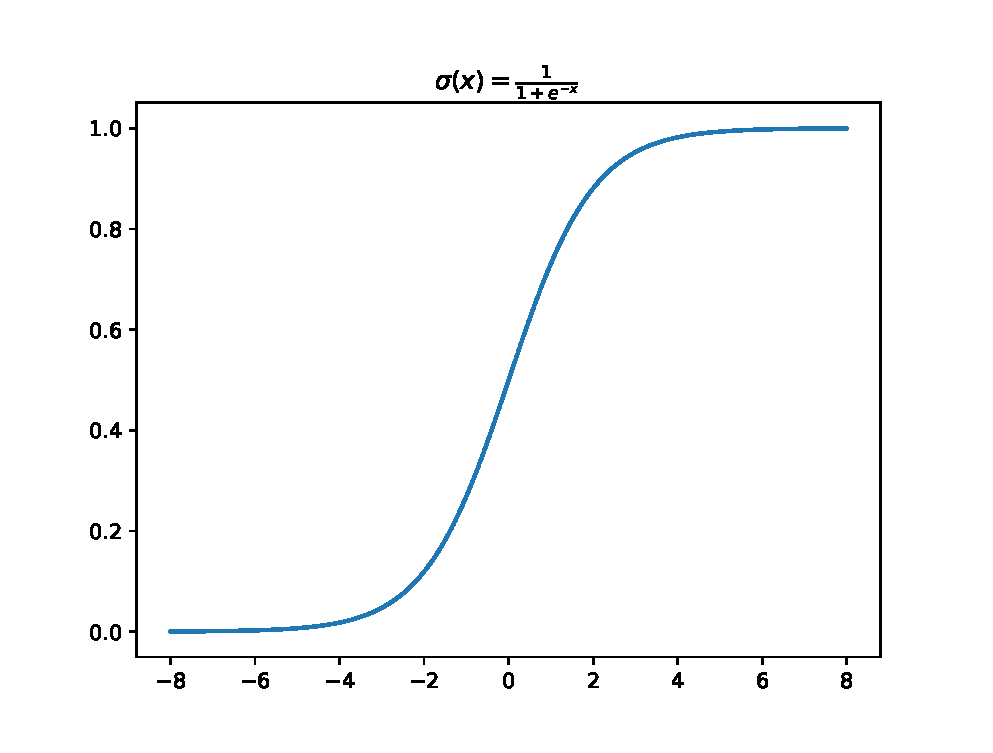
\includegraphics[width=\textwidth, trim=15 20 15 20, clip]{sigmoid.eps}
    \caption{Sigmoid}
    \label{fig:sigmoid}
  \end{figure}
  为此,首先需要定义损失函数,用以评估在回归过程中产生的偏差,即$Loss=
  \frac{1}{n}\sum\limits_i^n (y_i-y_i')^2$. 误差将指导参数的更新,在梯度下降算法中,使用损失从而计算参数更新的量,我们有:$$w := w -\eta \frac{\partial Loss}{\partial w}$$ $$b := b - \eta \frac{\partial Loss}{\partial b}$$
  其中$\eta$为学习率,为超参数。

  问题的核心在于,通过损失计算梯度,以确定参数更新的方向及更新量。根据梯度的计算方式,则有
  $$
  \begin{aligned}
    \frac{\partial Loss}{\partial w} &=  \frac{\partial}{\partial w} \left(\frac{1}{n} \sum _{i=1}^n (y-y')^2 \right) = \frac{\partial}{\partial y'} \left(\frac{1}{n} \sum _{i=1}^n (y_i-y_i')^2 \right) \times \frac{\partial y'}{\partial w} \\ 
    &= \frac{1}{n} \left(\sum_{i=1}^n 2(y-y')(-1) \right) \times \frac{\partial}{\partial w} \left( \frac{1}{1 + \exp(-(wx+b))} \right) \\ 
    &= -\frac{2}{n}\sum_{i=1}^n (y-y') \times -\frac{1}{(1+\exp(-(wx+b)))^2} \times -x\exp(-(w x+b)) \\ 
    &= -\frac{2}{n} \sum_{i=1}^n (y-y') \times x\frac{\exp(-(wx+b))}{(1+\exp(-(wx+b)))^2} \\ 
    &= -\frac{2}{n} \sum_{i=1}^n (y-y') \times x \frac{\exp(-(wx+b)) + 1 - 1}{(1+\exp(-(wx+b)))^2} \\ 
    &= -\frac{2x}{n} \sum_{i=1}^n (y-y') \times \left(\frac{1}{1+\exp(-(wx+b))} - \frac{1}{\left(1+\exp(-(wx+b))\right)^2} \right) \\ 
    &= -\frac{2x}{n}\sum_{i=1}^n (y-y') \left(\sigma(w x+b)(1-\sigma(w x+b))\right) \\ 
    &= -\frac{2x}{n}\sigma(1-\sigma) \sum_{i=1}^n (y-y')
  \end{aligned}
  $$

  \textbf{例:} 现拟合一个线性回归模型,其函数为$f(x;\theta)=g(\theta^\top x + b)$,根据最大似然估计方法,求$\theta$的更新梯度。

  \textbf{解:} 设模型的输出值为$y'$,真实值为$y$,则定义偏差为$P(\varepsilon^i)$表示对于第$i$个样本误差为$\varepsilon$的概率,其中$\varepsilon = y-y'$。对于所有的样本,其误差最终将服从均值为0,方差为$\sigma^2$的正态分布,即$P(\varepsilon^i)\sim \mathbb{N}(0, \sigma^2)$。由于$\theta$为参数,则使用最大似然估计求的$\theta$的估计值。

  似然函数:$L(\theta)=\prod\limits_i P(\varepsilon^i)$,根据似然函数写出对数似然函数为:$l(\theta)=\ln \prod\limits_i P(\varepsilon^i)=\sum\limits_i \ln P(\varepsilon^i)$

  为估测参数$\theta$,则需最大化对数似然,即
  $$
  \begin{aligned}
    &\arg\max\limits_\theta \sum\limits_i \ln P(\varepsilon^i)= \arg\max\limits_\theta \sum\limits_i \ln \frac{1}{\sqrt{2\pi}\sigma} e^{-\frac{(\varepsilon^i)^2}{2\sigma^2}} \\ 
    =& \arg\max\limits_\theta -n\ln \left(\sqrt{2\pi} \sigma \right) + \sum_i \left(-\frac{(\varepsilon^i)^2}{2\sigma^2}\right) \\ 
    = & \arg\max\limits_\theta \left(-n\ln \left(\sqrt{2\pi} \sigma \right) - \frac{1}{2\sigma^2}\sum_i (y^i-\theta^\top x^i + b)^2 \right)
  \end{aligned}
  $$
  需要最大化$l(\theta)$,则只需最小化$\frac{1}{2}\sum_i (y^i-\theta^\top x^i + b)^2$即可,则目标函数变为$\arg\min\limits_\theta \frac{1}{2}\sum_i (y^i-\theta^\top x^i + b)^2$,若将$b=\theta_0$,则目标函数为$\arg\min\limits_\theta \sum\limits_i \frac{1}{2}(y^i-\theta^\top x^i)^2=\arg\min\limits_\theta \sum\limits_i (y^i-\theta^Tx^i)^\top(y^i-\theta^Tx^i)$。对目标函数进行求导,或利用梯度下降算法,可得最终参数值。

  \textbf{例:} 求方程式$\frac{1}{N}\sum\limits_{i=1}^N \ln(1+\exp(-y_iw^\top x_i))$的梯度表达式。

  \textbf{解:} 
  $$
  \begin{aligned}
    \nabla &=-\frac{1}{N} \frac{\partial}{\partial w} \sum\limits_{i=1}^N \left(\ln (1 + \exp(-y_i w^\top x_i))\right) \\ 
    &= -\frac{1}{N} \sum_{i=1}^N \frac{\partial \ln \sigma}{\partial \sigma} \times \frac{\partial \sigma}{\partial w} = -\frac{1}{N} \sum_{i=1}^N  \frac{1}{\sigma} \times \frac{\partial \sigma(y_iw^\top x_i)}{\partial y_iw^\top x_i} \times \frac{\partial y_iw^\top x_i}{\partial w} \\ 
    &= -\frac{1}{N} \sum_{i=1}^N  \frac{1}{\sigma} \times \sigma(y_i w^\top x_i)(1-\sigma(y_i w^\top x_i)) x_i y_i \\ 
    &= -\frac{1}{N} \sum_{i=1}^N (1-\sigma(y_i w^\top x_i))x_i y_i = -\frac{1}{N} \sum_{i=1}^N \sigma(-y_i w^\top x_i)x_i y_i
  \end{aligned}
  $$

  \section{EM算法}
  现有三个硬币$A, B,C$,其朝上的概率分别为:$\pi, p, q$,采用如下规则进行抛掷:首先抛掷硬币$A$,根据硬币$A$的结果,若正面则选择$B$,反面则选择$C$。再次抛掷所选硬币,若为正面,则记为1,反面则记为0. 现有一组硬币序列为:
  $$1,1,0,1,0,0,1,0,1,1$$
  求三块硬币朝上的概率。

  \textbf{解}:
  设该硬币模型为:$\theta (\pi, p, q)$,其中模型被称为$\theta$,参数为$\pi, p, q$。记观测序列为$\mathbf{Y}=(Y_1, Y_2, Y_3,\cdots, Y_n)^{\mathop{T}}$,且$Y_n \in \{0, 1\}$. 记隐藏状态第一块硬币的状态为$\mathbf{Z}=(Z_1, Z_2, Z_3, \cdots, Z^n)^{\top}$,且$Z_n \in \{0, 1\}$. 

  根据观测序列,可计算$P(Y_n|\theta)$,而观测值,同时也依赖于第一块硬币的状态,则可得出,
  $$P(Y_n|\theta)=\sum_{Z_n \in \{0, 1\}}P(Y_n,Z_n|\theta)=\sum_{Z_n \in \{0, 1\}} P(Z_n|\theta)P(Y_n|Z_n,\theta)$$
  由$Z_n \in \{0, 1\}$可知,$P(Z_n=1|\theta)=\pi, P(Z_n=0|\theta)=1-\pi, P(Y_n|Z_n=1,\theta)=p^{y}(1-p)^{(1-y)},  P(Y_n|Z_n=0,\theta)=q^{y}(1- q)^{(1-y)}$. 由此可得,
  $$
  \begin{aligned}
    P(Y_n|\theta) &= P(Z_n=1|\theta)P(Y_n|Z_n=1,\theta)+P(Z_n=0|\theta)P(Y_n|Z_n=0,\theta) \\ 
    &= \pi p^y (1-p)^y + (1-\pi)^{(1-y)} q^y (1-q)^{(1-y)}
  \end{aligned}
  $$
  其中,$y$为当前样本的观测值,即$y\in \{0, 1\}$,

  为求三块硬币朝上的概率,即需要获得参数$\pi, p, q$的值,可使用最大似然估计,即
  $$\arg\max_{\theta} \log P(\mathbf{Y}|\theta)=\arg\max_{\theta} \log\prod_{i=1} ^n (\pi p^{y_i} (1-p)^{y_i} + (1-\pi)^{1-y_i} q^{y_i} (1-q)^{1-y_i}).$$
  此式无解析解,因此需要采用其他算法求解。
  
  在EM算法中,采用迭代的方式求解所需参数,该算法通过E步与M步分别求解。

  \textbf{E步:}计算在第$i$次迭代后,模型$\theta(\pi^(i), p^{(i), q^{(i)}})$下的观测结果$y_j$来自硬币$B$的观测结果的概率为:
  $$
  \mu_j^{(i+1)} = \frac{\pi^{(i)} \left(p^{(i)}\right)^{y_j} (1-p^{(i)})^{y_j}}{\pi^{(i)} \left(p^{(i)}\right)^{y_j} (1-p^{(i)})^{y_j} + \left(1-\pi^{(i)}\right)^{(1-y_j)} \left(q^{(i)}\right)^{y_j} (1-q^{(i)})^{(1-y_j)}}
  $$

  \textbf{M步:} 经过E步后,可经过M步对第$i+1$次迭代的参数进行更新:
  \begin{equation}
    \pi^{(i+1)} = \frac{1}{n}\sum_{j=1}^n \mu_j^{(i+1)}
  \end{equation}
  \begin{equation}
    p^{(i+1)} = \frac{\sum_{j=1}^n \mu_j^{(i+1)}y_j}{\sum_{j=1}^n \mu_j^{(i+1)}}
  \end{equation}
  \begin{equation}
    q^{(i+1)} = \frac{\sum_{j=1}^n \left(1-\mu_j^{(i+1)}\right)y_j}{\sum_{j=1}^n \left(1-\mu_j^{(i+1)}\right)}
  \end{equation}

  \paragraph{总结} EM算法是通过给定参数的初值,通过对样本进行逐步迭代,直至参数收敛时得到最终参数的估计值的算法。

  \subsection{EM算法的推导}
  给定一组观测数据$x_2,x_2,\cdots, x_m$,切各观测样本相互独立,为拟合该观测数据的模型$p(x,z)$,便需要获取到模型的参数。其中$z$为隐藏变量,不可有观测数据观测得出。

  根据描述,可将模型描述为$p(x;\theta)$,即参数为$\theta$的一个概率模型。可以尝试将其写为条件概率的形式,即$p(x|\theta)$。根据联合概率分布,可以将隐含参数引入,得$p(x|\theta)=\sum\limits_zp(x,z|\theta)$. 根据最大似然估计,对模型中的参数进行估计,则有
  \begin{equation}
    \ell(\theta) = \sum_{i=1}^m \ln \sum\limits_zp(x,z|\theta)
    \label{eq:max-likelyhood-em}
  \end{equation}
  由公式\ref{eq:max-likelyhood-em}可知,若采用最大似然估计方法,需要对$\ell (\theta)$求偏导,而根据对数函数的导数$\ln '(x) = \frac{1}{x}$,因此对“\textbf{和的对数}”求导结果复杂,无法求解。

  为此引入一个分布为$Q(z)$,其中$z$为随机变量,而$Q(z)$为随机变量的概率密度函数。则有$\sum\limits_{i=1}^m Q(z_i) = 1$,此时$z$为离散型随机变量,若$z$为连续性随机变量,则应为$\int_{-\infty}^{\infty} Q(z) = 1$. 
  
  根据公式\ref{eq:max-likelyhood-em},可在分子分母同时乘以一个函数$Q(z)$,即
  \begin{equation}
    \ell(\theta) = \sum_{i=1}^m \ln \sum_z Q(z) \frac{p(x,z|\theta)}{Q(z)}
    \label{eq:e-step1}
  \end{equation}
  由$\sum\limits_{i=1}^m Q(z_i) = 1$,则可将$Q(z)$视为$p(x)$,根据\ref{subsec:e-jensen}节中期望的定义,可将$\frac{p(x,z|\theta)}{Q(z)}$视为$g(x)$,因此可将公式\ref{eq:e-step1}进行变换为:
  \begin{equation}
    \ell (\theta) = \sum_{i=1}^m \ln E(\Lambda), E(\Lambda) = \sum_z Q(z) \frac{p(x,z|\theta)}{Q(z)}
  \end{equation}
  根据\ref{subsec:e-jensen}节中Jensen不等式,由于对数函数的二阶导为$-\frac{1}{x^2} < 0$,则对数函数为凹函数,故有$E(f(x)) \leq f(E(X))$. 即 $\ln E(\Lambda) \geq E(\ln \Lambda) $即$\ln \sum\limits_z Q(z) \frac{p(x,z|\theta)}{Q(z)} \geq \sum\limits_z Q(z) \ln \frac{p(x,z|\theta)}{Q(z)} $
  则$\ell (\theta)$进一步转化为:
  \begin{equation}
    \ell(\theta) \geq \sum _{i=1} ^m \sum _z Q(z) \ln \frac{p(x,z|\theta)}{Q(z)}
    \label{eq:em-m-step1}
  \end{equation}
  公式\ref{eq:em-m-step1}将“\textbf{和的对数}”转化为了“\textbf{对数的和}”,对该式求导将更加方便求解。

  其中根据Jensen不等式,当$X=E(X)$时等式成立,即随机变量为一个常数,则有$\frac{p(x,z|\theta)}{Q(z)}=c$,进一步变换,可有$\sum\limits_z p(x,z|\theta) = \sum\limits_z Q(z) \frac{p(x,z|\theta)}{Q(z)}=\sum Q(z)c$,由于$\sum\limits _z Q(z)=1$,则有$\sum\limits_z p(x,z|\theta) = c$. 进一步可推$Q_i(z^{(i)})=p(z^{(i)}|x(i),\theta) = \frac{p(z^{(i)}, x^{(i)}|\theta)}{\sum\limits_z p(z, x^{(i)}|\theta)}$
  

  \paragraph{总结} EM算法分为两步,一部分为求期望,该期望指的是引入隐含变量的概率分布,求期望,并以该概率分布的迭代值作为隐含参数的后验概率。再通过后验概率最大化似然函数,调整参数$\theta$.
  \begin{enumerate}
    \item 引入隐变量的分布,即$Q(z)$,并且$Q(z^{(i)}) := \frac{p(x^{(i)}, z^{(i)} | \theta)}{\sum\limits_z p(x^{(i)}, z | \theta)}$ \footnote{$i$指每次迭代,下同。};
    \item 根据$Q(z^{(i)})$,最 大化$\sum\limits _{i=1} ^m \sum\limits _z Q(z) \ln \frac{p(x,z|\theta)}{Q(z)}$, 并迭代进行。
  \end{enumerate}

  \section{机器学习}
  \section{深度学习}\label{sec:nn-dl}

\subsection{前向传播}

设有训练样本为$\mathbf{X}$,其经过特征提取后共有$m$个特征,则对于任意样本,有$\mathbf{X} \in \mathbb{R}^{m}$,通常样本向量为列向量,行数即为其特征维度的大小。神经网络结构,如图\ref{fig:nn}所示,对于多层神经网络,其包含输入层、隐藏层、输出层。
\begin{figure}[hbp]
  \centering
  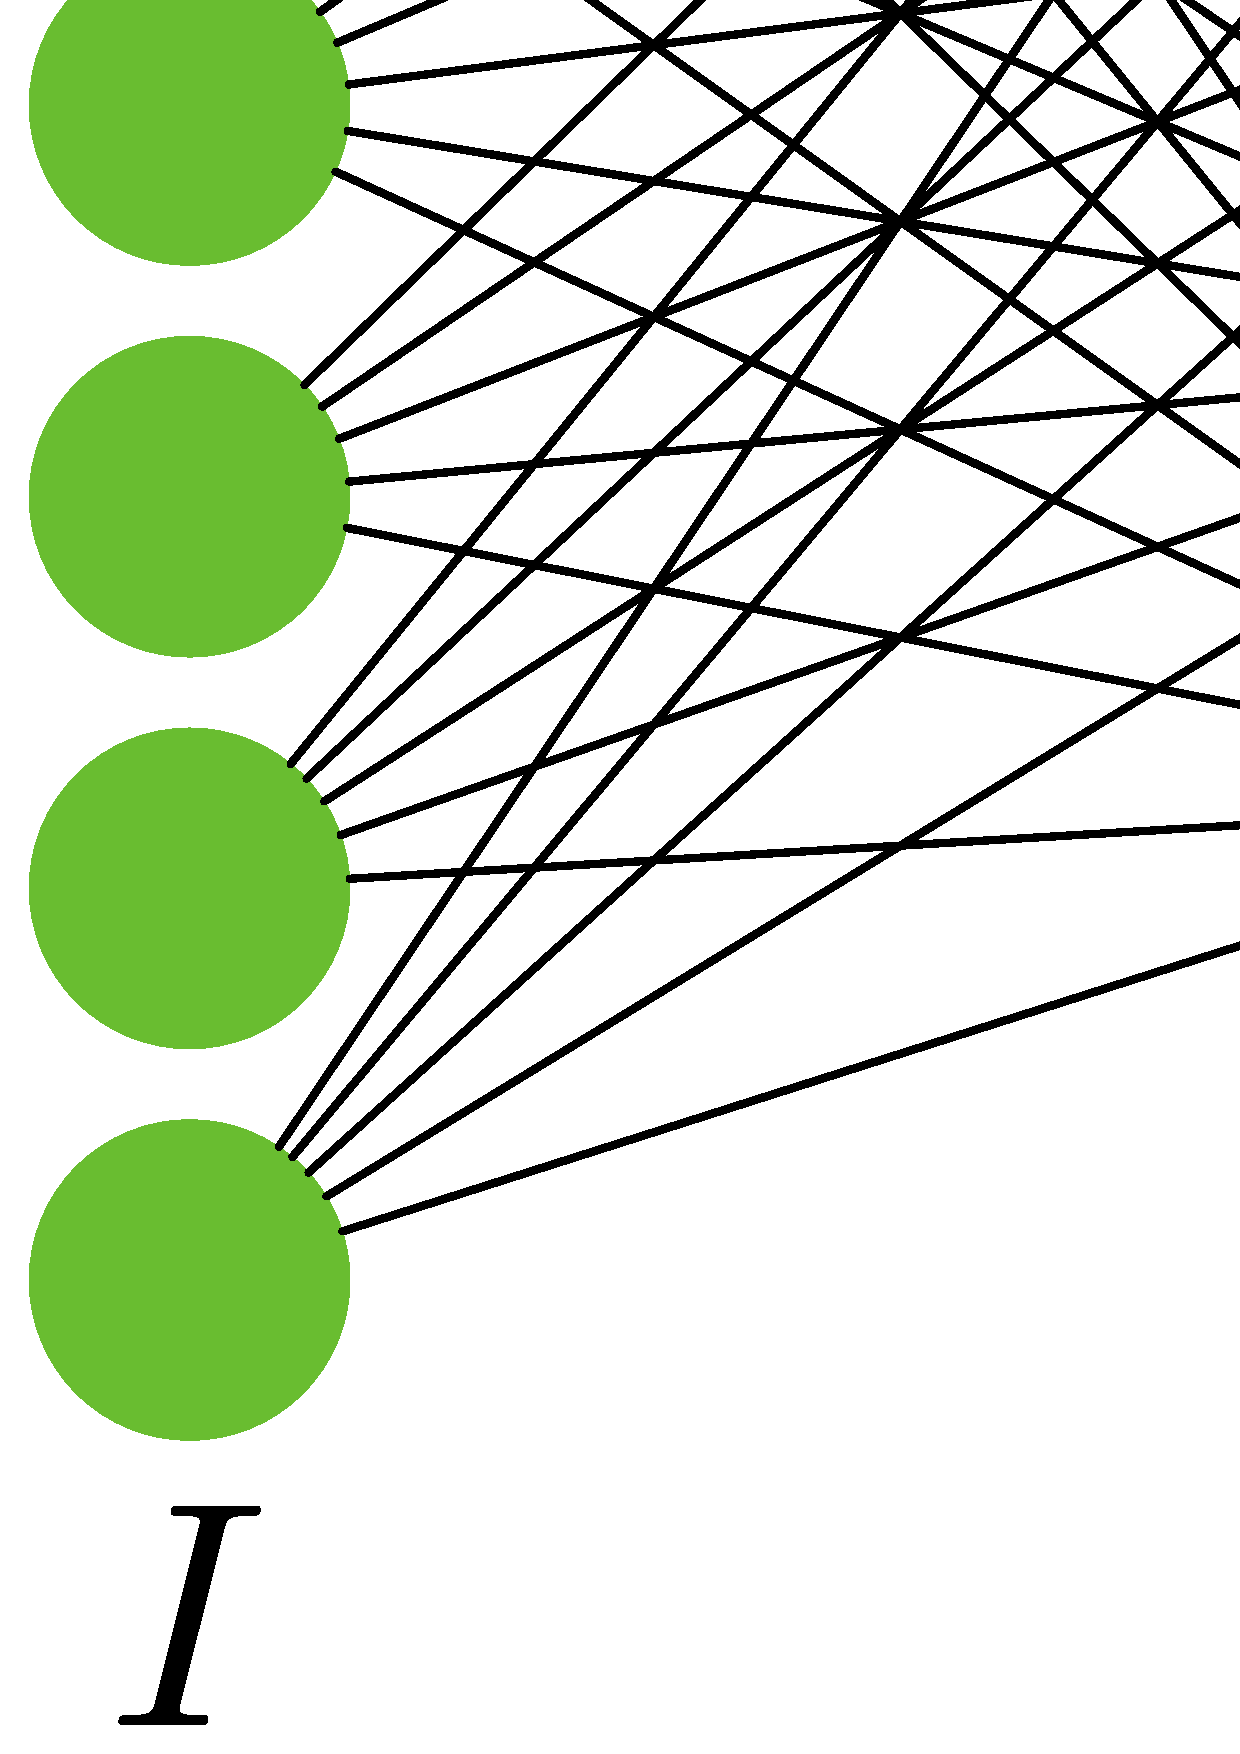
\includegraphics[width=.7\textwidth]{figures/nn.pdf}
  \caption{神经网络示意图}
  \label{fig:nn}
\end{figure}

神经网络通过前向传播得出模型的预测结果,即对结果的拟合。其过程如下,对于输入$\mathbf{X}$,其输入到第一层隐藏层,进行线性激活:$\mathbf{Z}^{[1]} = \mathbf{W}^{[1]} \times \mathbf{X} + b^{[1]}$,由于多次线性变换的结果仍未线性变换,则需要在线性激活函数后加入非线性函数再次激活。则对于第1层隐藏层,其激活后的输出结果为$\mathbf{A}^{[1]}=\sigma (\mathbf{Z}^{[1]})$,其中$\sigma$为激活函数。

对于从第$l$层隐藏层到第$l+1$层隐藏层,则$l+1$层输入为$l$层的激活后输出$\mathbf{A}^{[l]}$,则前向传播过程为:
\begin{equation}
  \mathbf{Z}^{[l]} = \mathbf{W}^{[l]} \times \mathbf{A}^{[l - 1]} + b^{[l]}
  \label{eq:linear-activation}
\end{equation}
\begin{equation}
  \mathbf{A}^{[l]} = \sigma (\mathbf{Z}^{[l]})
  \label{eq:nonlinear-activation}
\end{equation}
在公式\ref{eq:linear-activation}中,$\mathbf{W} \in \mathbb{R}^{n \times m}$,其中$n$为当前隐藏层的神经元个数,$m$为上一层神经元个数,则$\mathbf{Z}^{[l]} \in \mathbb{R}^{n}$为新的列向量。则说明,在神经网络中,根据不同的权重,将原始的特征有$m$个逐渐提取为$n$个更加有效的特征,便于拟合一个$x\rightarrow y$的映射。在对于输出层$L$,则其最终的输出结果即为$\mathbf{A}^{[L]}$,则有$\hat{y}=\mathbf{A}^{[L]}$. 则$\hat{y}$即为模型给出的最终预测结果,或拟合结果。可知,在训练初期,神经网络通过随机初始化权重$\mathbf{W}$从而得出预测结果,其结果必定与真是结果存在较大偏差,因此需要对参数进行更新,而参数更新的结果即为反向传播过程。在更新参数之前,我们需要首先定义损失函数(即代价函数,损失函数),用于衡量预测值与真实值之间的差异。

在考虑代价函数之前,可以推导,为何多次线性变换的结果仍为线性变换,设在神经网络中,各层参数采用$\boldsymbol{\theta}^{[l]}$表示,其中$b$也为$\boldsymbol{\theta}$中的某一维度,则有:
\begin{enumerate}[label=第\arabic{*}层: ,itemindent=36pt]
  \item $\mathbf{Z}^{[1]} = \boldsymbol{\theta}^{[1]} \times \mathbf{X}$; 
  \item $\mathbf{Z}^{[2]} = \boldsymbol{\theta}^{[2]} \times \mathbf{Z}^{[1]} = \boldsymbol{\theta}^{[2]} \times \boldsymbol{\theta}^{[1]} \times \mathbf{X}$; 
  \item[第n层:] $\mathbf{Z}^{[n]} = \boldsymbol{\theta}^{[n]} \times \mathbf{Z}^{[n-1]} = \boldsymbol{\theta}^{[n]} \times \boldsymbol{\theta}^{[n-1]} \times \cdots \times \boldsymbol{\theta}^{[1]} \times \mathbf{X} = \prod\limits _{i=1}^n \boldsymbol{\theta}^{[i]} \times \mathbf{X}$
\end{enumerate}

由上可知,$\prod\limits _{i=1}^n \boldsymbol{\theta}^{[i]}$可等价为一个参数$\boldsymbol{\theta}$,因此多层线性变换其结果仍为线性变换。

\subsection{代价函数}

通常可以将代价函数定义为$J(\boldsymbol{\theta})$,其中$\boldsymbol{\theta}$为多维参数,包含了$\mathbf{W}$与$b$,因为$b$可视为$\boldsymbol{\theta}_0$, 其中$\boldsymbol{\theta}^{[l]}$表示第$l$层的参数。

\subsubsection{Categorical Cross Entropy}
\begin{equation}
  H(y, \hat{y})=-\sum_{i} y_{i} \log \hat{y}_{i}
  \label{eq:cost-cross-entropy}
\end{equation}
公式\ref{eq:cost-cross-entropy}在\ref{subsec:cross-entropy}节中已有推导,其来自信息论用于衡量两个数据分布之间的差异。在公式\ref{eq:cost-cross-entropy}中,$\hat{y}_{i}$则为预测值,而$y_i$则为真实值。

\subsubsection{Softamx Cross Entropy}
同公式\ref{eq:cost-cross-entropy}. 不同的在于
$$\hat{y}_i=\operatorname{softmax}\left(z_{j}\right)=\frac{e^{z_{j}}}{\sum \limits_{j} e^{z_{j}}}$$
则$\sum \limits_j \hat{y}_j= 1$. 

\subsubsection{Binary Cross Entropy}
根据公式\ref{eq:cost-cross-entropy}, 对于二分类问题,其只需要通过$sigmoid$激活函数输出一个$(0,1)$的值即可,其$\hat{y} \in (0, 1)$. 则其损失函数可定义为:
\begin{equation}
  J(\boldsymbol{\theta})=-[y \cdot \log (\hat{y})+(1-y) \cdot \log (1-\hat{y})]
  \label{eq:cost-binary-cross-entropy}
\end{equation}


\subsubsection{Weighted Cross Entropy}
经过加权的交叉熵损失函数,其可用于处理不平衡分类的损失计算,其定义为:
\begin{equation}
  J(\boldsymbol{\theta}) = -\sum \limits _i  w_i y_i \log \hat{y}_i
  \label{eq:cost-weighted-cross-entropy}
\end{equation}
其中$w_i$即为每个类别的权重,为超参数。

\subsubsection{Mean Square Loss}
\begin{equation}
  M S E=\frac{1}{n} \sum_{i=1}^{n}\left(\hat{y}_{i}-y_{i}\right)^{2}
  \label{eq:cost-mse}
\end{equation}
\subsubsection{Hinge Loss}

\begin{equation}
  J(\boldsymbol{\theta})=\max (0,1-y * \hat{y})
\end{equation}

\subsubsection{ROC AUC Score}

\subsubsection{Weak Softmax Cross Entropy 2d}

\subsubsection{Contrastive Loss}
\begin{equation}
  J(\boldsymbol{\theta})=\frac{1}{2 N} \sum_{n=1}^{N} y d^{2}+(1-y) \max (\operatorname{margin}-d, 0)^{2}
\end{equation}
其中$d=\left\|x_{i}-x_{j}\right\|_{2}$

\subsection{梯度下降}
梯度下降是最优化求解的一种方法,对于一个优化函数,根据其梯度的方向,更新参数,便可使得代价函数达到最小值或最大值(梯度上升)。
其中梯度即为函数在某一方向上的偏导数。如,$\nabla _a J$表示代价函数$J$对于参数$a$的梯度。

在神经网络中,有参数为$\boldsymbol{\theta}$,则可定义梯度为$\nabla _{\boldsymbol{\theta}} J$. 而梯度更新的方式则为:$\boldsymbol{\theta} := \boldsymbol{\theta} - \eta \nabla_
{\boldsymbol{\theta}} J$,其中$\eta$为学习率,为神经网络的超参数。

\subsubsection{反向传播推导}
反向传播,用于从输出层,逐步向隐藏层各层反向传播,使用梯度下降方法,计算梯度,更新参数,使模型拟合能力更强。
对于输出层$L$,其输出为$\mathbf{A}^{[L]}$,定义损失函数为$J(\boldsymbol{\theta})$,则参数$\mathbf{W}$的梯度为:
\begin{equation}
  \nabla _{w^{[L]}} J = \frac{\partial J}{\partial \mathbf{W}^{[L]}}
  \label{eq:nabla_W}
\end{equation}
令$\delta ^{[L]} = \frac{\partial J}{\partial \mathbf{Z}^{[L]}} = \frac{\partial J}{\partial \mathbf{A}^{[L]}} \odot \frac{\partial \mathbf{A}^{[L]}}{\partial \mathbf{Z}^{[L]}} = \nabla _{\mathbf{A}^{[L]}} J \odot \sigma ' \left(\mathbf{Z}^{[L]}\right)$. 由损失函数的定义可知,损失为一个常数,为标量,则其对一个向量进行微分时,值仍为一个向量。

对上述推导进行推广可知,对于$l$层的每个神经元,其损失来自于下一层与该神经元连接的所有神经元的输出,即:
$$
\frac{\partial J}{\partial \mathbf{A}^{[l]}} = \frac{\partial J}{\partial \mathbf{A}^{[l + 1]}} \times \frac{\partial \mathbf{A}^{[l + 1]}}{\partial \mathbf{Z}^{[l + 1]}} \times \frac{\partial \mathbf{Z}^{[l + 1]}}{\partial \mathbf{A}^{[l]}} = {\mathbf{W} ^{[l + 1]}}^\top \times \delta ^{[l+1]}
$$
根据$\delta ^{[L]}$的定义,则有
\begin{equation}
\delta ^{[l]} = \frac{\partial J}{\partial \mathbf{Z}^{[l]}} = {\mathbf{W} ^{[l + 1]}}^\top \times \delta ^{[l + 1]} \odot \sigma ' \left(\mathbf{Z}^{[l]}\right)
\label{eq:theta_l_with_l_plus_1}
\end{equation}

则根据公式\ref{eq:nabla_W},有
\begin{equation}
  \begin{aligned}
    \nabla _{w^{[l]}} J &= \frac{\partial J}{\partial \mathbf{W}^{[l]}} = \frac{\partial J}{\partial \mathbf{Z}^{[l]}} \times \frac{\partial \mathbf{Z}^{[l]}}{\partial \mathbf{W}^{[l]}} = \delta^{[l]} \times {\mathbf{A}^{[l - 1]}}^\top \\ 
  \end{aligned}
  \label{eq:nabla_W_l}
\end{equation}
同理,对于偏置,则有
\begin{equation}
  \begin{aligned}
    \nabla _{b^{[l]}} J &= \frac{\partial J}{\partial b^{[l]}} = \frac{\partial J}{\partial \mathbf{Z}^{[l]}} \times \frac{\partial \mathbf{Z}^{[l]}}{\partial b^{[l]}} = \delta ^{[l]}
  \end{aligned}
  \label{eq:nabla_b_l}
\end{equation}

可以根据维度,对上述推导,可通过维度进行验证,如$\delta^{[l]} \times {\mathbf{A}^{[l - 1]}}^\top$,对于$l$层设有$n$个神经元,而$m$层有$n$个神经元,则$\delta^{[l]}$为$n \times 1$,而${\mathbf{A}^{[l - 1]}}^\top$为$1\times m$,则最终结果为$n \times m$维,与$\mathbf{W}^{[l]}$维度相同。

\subsubsection{优化方法(权重衰减)}

\section{卷积神经网络}

\subsection{前向传播}
卷积神经网络前向传播通常包含三部分:卷积层、池化层、全连接层,如图\ref{fig:vgg16-net},其包含5个卷积层,卷积层后包含了2个全连接层,其中省略了池化层。在卷积网络中,使用$\odot$表示卷积运算,指对应元素相乘再求和,其表示一种element-wise操作。由于卷积操作能够提取原始矩阵中的信息,但卷积核在提取过程中,仍有重复计算的部分,因此引入了池化层,来减小下一层的计算量,常用的池化操作有Max-Pooling与Avg-Pooling。池化操作通常只有$filter\_size$及$stride$参数,而无$padding$参数,并且都为超参数,无需要学习的参数。
\begin{figure}[htbp]
  \centering
  \includegraphics[width=\textwidth]{figures/vgg16.pdf}
  \caption{VGG-16}
  \label{fig:vgg16-net}
\end{figure}

在卷积层中,含有的参数为:1) $filter\_size$,即卷积核(或滤波器)大小;2) $stride$,即步长;3) $padding$,即填充模式,及填充的大小。卷积层,通过使用滤波器,在输入数据中进行扫描,进行卷积运算,得到一个输出值,并使用$stride$为步长,向右或向下移动卷积核,以提取下一个特征\footnote{卷积核大小通常使用奇数,卷积核个数决定了输出的通道数。}。
\begin{figure}[htbp]
  \centering
  \includegraphics[width=.9\textwidth]{figures/convolutional-operation.pdf}
  \caption{卷积运算,使用$3\times 3$卷积核以$2$为步长no-padding,对$6\times 6$输入进行卷积,得$4\times 4$输出}
  \label{fig:convolotional-operation}
\end{figure}
如图\ref{fig:convolotional-operation},使用$3\times 3$的卷积核在$6 \times 6$的输入上进行扫描,并进行卷积运算,可得到一个值为-4,如此向右以2为步长移动,可得出第二个值。如此迭代,便可生成一个新的$2 \times 2$的输出。同时在卷积网络中,经过卷积运算得到的输出还需经过非线性激活函数,才可作为下一层的输出。在卷积神经网络中,通常使用ReLU函数进行激活。

由此,可推出卷积运算,输入与输出大小的关系:
$$
  size = \left\lfloor \frac{{size}_{prev} + 2pad - filter\_size}{stride} \right\rfloor + 1
$$
由此,经过卷积运算后,若无padding,则原输入的大小将会被压缩。对于存在padding的情况,则通常有两种padding类型:SAME和VALID。SAME-padding是指经过padding后,输出的大小与输入大小保持一致,并在需要补充边界的地方,填充0。因此,若采用SAME-padding方式,则
$$
  \begin{aligned}
    size_{prev} = \left\lfloor \frac{{size}_{prev} + 2pad - filter\_size}{stride} \right\rfloor + 1 \\ 
    pad = \frac{(stride - 1)size - stride +filter\_size}{2}
  \end{aligned}
$$
对应的,若采用VALID方式,则卷积核会跳过大小不满足的区域。

池化层,实际上可视为一种特殊的卷积运算,只是卷积运算不同。对于最大池化,其同样使用一个卷积核对输出进行扫描,并对区域内的值选择最大值作为该区域的最终值。而对于平均池化,则使用区域内的均值作为最终值。其中较常用的池化方法为最大池化。

在卷积网络中,卷积核的个数,决定了输出的通道数量。对于$l$层的输入,其为$\mathbf{X} \in \mathbb{R}^{n_H^{[l-1]} \times n_W^{[l-1]} \times n_C^{[l-1]}}$,而卷积核则为$\mathbf{F} \in \mathbb{R}^{size^{[l]} \times size^{[l]} \times n_C{[l-1]} \times n_C{[l]}}$,最终得到输出为$\mathbf{Y} \in \mathbb{R}^{n_H ^{[l]} \times n_W ^{[l]} \times n_C^{[l]}}$。

在经过卷积后,卷积神经网络已提取足够多的可用特征,便可将所有的特征,作为全连接神经网络中,实现结果的预测,如分类问题或回归问题等。全连接层的加入,由任务决定,可有可无。

综上,可对卷积神经网络的前向传播进行总结:
\paragraph{卷积:}
设输入为$\mathbf{X} \in \mathbb{R}^{n_H \times n_W \times n_C}$卷积核大小为$p \times p \times n_C$,个数为$n_C '$,步长为$stride$,采用VALID即no-padding方式,则最终输出结果为$\mathbf{Y}$,且$\mathbf{Y}_{i,j,c} = \mathbf{X}_{(i-1)stride:(i-1)stride+p-1,(j-1)stride:(j-1)stride+p-1,:c} \odot \mathbf{F}_{:,:,:,c}, i \in \{1, 2, \cdots, \left\lfloor\frac{n_H - p}{stride}\right\rfloor + 1\}, j \in \{1, 2, \cdots, \left\lfloor\frac{n_W - p}{stride}\right\rfloor + 1\}, c \in \{1, 2, \cdots, n_C '\}$
\paragraph{池化:}
由于在卷积神经网络中,先池化再激活,与先激活再池化的结果一致\footnote{由于激活函数一般属于递增函数。},而池化对卷积结果进行了下采样,缩小了计算规模,因此在池化后再进行激活,其效率更高。设经过卷积后的输出为$\mathbf{Z} \in \mathbb{R}^{n_H \times n_W \times n_C}$,采用步长为$stride$,大小为$p\times p$的卷积核进行池化,则有输出$\mathbf{Z}'$,且$\mathbf{Z}'_{i,j,c} = \max \left(\mathbf{Z}_{(i - 1)stride:(i-1)stride + p - 1,(j - 1)stride:(j-1)stride + p - 1, c}\right)$,经过激活函数后,得到$\mathbf{A} = \operatorname{ReLU}(\mathbf{Z}')$. 
\paragraph{全连接层(可选):}
见\ref{sec:nn-dl}节。

\subsection{梯度下降}
同\ref{sec:nn-dl}节中对梯度下降的描述相同,卷积神经网络也通过梯度下降的方式,来最优化调整模型,并更新参数,使模型的拟合能力增强。
而不同的是,在普通的全连接神经网络中,各隐藏层之间的结构相同,即当前层的一个神经元与下一层的所有神经元皆有连接。而卷积神经网络中,卷积层、池化层、全连接层,属于不同的隐藏层结构,其在不同层的前向传播计算过程不同,那么梯度计算方法也不同。
\subsubsection{反向传播推导}
在推导反向传播的过程时,分四个阶段分别进行:1) 输出层至全连接层;2) 全连接层至池化层;3) 池化层至卷积层; 4) 卷积层至上一层(池化层)。反向传播与全连接神经网络相似,因此需要基于公式\ref{eq:theta_l_with_l_plus_1}. 
\paragraph{1) 输出层至全连接层:}这部分同全连接网络相同,使用公式\ref{eq:theta_l_with_l_plus_1}、\ref{eq:nabla_W_l}、\ref{eq:nabla_b_l}即可。
\paragraph{2) 全连接层至池化层:}
根据前向传播可知,若池化层的下一层为全连接层,则池化层至全连接层没有参数,只进行了flatten操作。因此全连接层至池化层,只需将向量去flatten为原始形状即可,即$\mathbf{A}^{[l]} \in \mathbb{R}^{n_H \cdot n_W \cdot n_C \times 1} \rightarrow \mathbf{A}^{[l]} \in  \mathbb{R}^{n_H \times n_W \times n_C}$,因此基于公式\ref{eq:theta_l_with_l_plus_1},可将该过程表示为$\delta^{[l]} = \operatorname{unflattern}\left(\delta ^{[l + 1]}\right) \odot \sigma ' \left(^{[l]}\right)$
\paragraph{3) 池化层至卷积层:}本质上,池化层至卷积层在前向传播过程中,只是对卷积层进行了采样,无所需学习的参数,因此在这部分,需将池化层的结果重新去池化为卷积层的形状。池化操作通常包含两种:Max-Pooling及Avg-Pooling,对于Max-Pooling,在去池化的过程中,首先将池化层的结果使用0填充至上一层的规模,之后将在前向传播过程中所记录的最大值的位置,将至填充到新的矩阵中,如设池化所用核大小为$2\times 2$,得到输出:
$$
\delta_{k}^{l}=\left(\begin{array}{ll}{2} & {8} \\ {4} & {6}\end{array}\right)
$$
由于池化的核大小为$2 \times 2$,则对其进行填充,得到:
$$
\left(\begin{array}{llll}{0} & {0} & {0} & {0} \\ {0} & {2} & {8} & {0} \\ {0} & {4} & {6} & {0} \\ {0} & {0} & {0} & {0}\end{array}\right)
$$
设前向传播过程中,所记录的最大值位置为$(0,0), (1, 1), (1, 0), (1, 0)$,则将其还原,得到:
$$
\left(\begin{array}{llll}{2} & {0} & {0} & {0} \\ {0} & {0} & {0} & {8} \\ {0} & {4} & {0} & {0} \\ {0} & {0} & {6} & {0}\end{array}\right)
$$
若采用Avg-Pooling,则仅需将各个元素平均,分散即可,如:
$$
  \left(\begin{array}{cccc}{0.5} & {0.5} & {2} & {2} \\ {0.5} & {0.5} & {2} & {2} \\ {1} & {1} & {1.5} & {1.5} \\ {1} & {1} & {1.5} & {1.5}\end{array}\right)
$$

根据反向传播的关系$\delta ^{[l]} = \nabla _{\mathbf{A}^{[l]}} J \odot \sigma' \left(\mathbf{Z}^{[l]}\right)$,则有
$$
\nabla _{\mathbf{A}^{[l]}} J = \frac{\partial J}{\partial \mathbf{A}^{[l]}} = \frac{\partial J}{\partial \mathbf{Z}^{[l + 1]}} \cdot \frac{\partial \mathbf{Z}^{[l + 1]}}{\partial \mathbf{A}^{[l]}} = \delta ^{[l + 1]} \cdot \frac{\partial \mathbf{Z}^{[l + 1]}}{\partial \mathbf{A}^{[l]}}
$$
不同的是,由于在池化层中,$\mathbf{Z}^{[l + 1]}$与${\partial \mathbf{A}^{[l]}}$的关系为一个池化过程,从$l$至$l+1$层时,产生了维度缩减,而池化层无待学参数,因此反向传播仅需将误差扩增到原始维度。因此$\frac{\partial \mathbf{Z}^{[l + 1]}}{\partial \mathbf{A}^{[l]}}$表示的应是对下一层的误差进行去池化,即$\delta ^{[l]} = \operatorname{unsample} \left(\delta ^{[l+1]}\right)\cdot \sigma' \left(\mathbf{Z}^{[l]}\right)$. 

\paragraph{4) 卷积层至上一层(池化层):}
为推导反向传播过程,应先观察正向传播的过程,其计算如图\ref{fig:conv-fp}:
\begin{figure}[htbp]
  \centering
  \includegraphics[width=.8\textwidth]{figures/convolutional-fp.pdf}
  \caption{卷积层正向传播}
  \label{fig:conv-fp}
\end{figure}
其计算结果可表示为:
$$
\begin{aligned}
  \mathbf{O}_{1,1} &= \mathbf{X}_{1,1}\mathbf{F}_{1,1} + \mathbf{X}_{1,2}\mathbf{F}_{1,2} + \mathbf{X}_{2,1}\mathbf{F}_{2,1} + \mathbf{X}_{2,2}\mathbf{F}_{2,2} \\
  \mathbf{O}_{1,2} &= \mathbf{X}_{1,2}\mathbf{F}_{1,1} + \mathbf{X}_{1,3}\mathbf{F}_{1,2} + \mathbf{X}_{2,2}\mathbf{F}_{2,1} + \mathbf{X}_{2,3}\mathbf{F}_{2,2} \\
  \mathbf{O}_{2,1} &= \mathbf{X}_{2,1}\mathbf{F}_{1,1} + \mathbf{X}_{2,2}\mathbf{F}_{1,2} + \mathbf{X}_{3,1}\mathbf{F}_{2,1} + \mathbf{X}_{3,2}\mathbf{F}_{2,2} \\
  \mathbf{O}_{2,2} &= \mathbf{X}_{2,2}\mathbf{F}_{1,1} + \mathbf{X}_{2,3}\mathbf{F}_{1,2} + \mathbf{X}_{3,2}\mathbf{F}_{2,1} + \mathbf{X}_{3,3}\mathbf{F}_{2,2} \\
\end{aligned}
$$
根据反向传播公式$\delta ^{[l]} = \nabla _{\mathbf{A}^{[l]}} J \odot \sigma' \left(\mathbf{Z}^{[l]}\right)$,进一步推导,对于$\nabla _{\mathbf{A}^{[l]}} J = \frac{\partial J}{\partial \mathbf{A}^{[l]}}$,则有
$$
\frac{\partial J}{\partial \mathbf{A}^{[l]}} = \frac{\partial J}{\partial \mathbf{Z}^{[l + 1]}} \cdot \frac{\partial \mathbf{Z}^{[l + 1]}}{\partial \mathbf{A}^{[l]}}
$$
根据前向传播结果,$\mathbf{A}^{[l]}$经过卷积运算,得到$\mathbf{Z}^{[l + 1]}$,因此对上述前向传播的过程进行微分,$2\times 2$的输出,将被还原为$3 \times 3$,并有
$$
\begin{aligned}
  \nabla_{\mathbf{X}_{1,1}} &= \frac{\partial \mathbf{O}_{1,1}}{\partial \mathbf{X}_{1,1}} = \frac{\partial}{\partial \mathbf{X}_{1,1}} \left( \mathbf{X}_{1,1}\mathbf{F}_{1,1} + \mathbf{X}_{1,2}\mathbf{F}_{1,2} + \mathbf{X}_{2,1}\mathbf{F}_{2,1} + \mathbf{X}_{2,2}\mathbf{F}_{2,2} \right) = \mathbf{F}_{1,1} \\
  \nabla_{\mathbf{X}_{1,2}} &= \frac{\partial \mathbf{O}_{1,1}}{\partial \mathbf{X}_{1,1}} + \frac{\partial \mathbf{O}_{1,2}}{\partial \mathbf{X}_{1,2}} = \mathbf{F}_{1,1} + \mathbf{F}_{1,2} \\ 
  \nabla_{\mathbf{X}_{1,3}} &= \frac{\partial \mathbf{O}_{1,2}}{\partial \mathbf{X}_{1,3}} = \mathbf{F}_{1,2} \\
  \nabla_{\mathbf{X}_{2,1}} &= \frac{\partial \mathbf{O}_{1,1}}{\partial \mathbf{X}_{2,1}} + \frac{\partial \mathbf{O}_{2,1}}{\partial \mathbf{X}_{2,1}} = \mathbf{F}_{2,1} + \mathbf{F}_{1,1} \\ 
  \nabla_{\mathbf{X}_{2,2}} &= \frac{\partial \mathbf{O}_{1,1}}{\partial \mathbf{X}_{2,2}} + \frac{\partial \mathbf{O}_{1,2}}{\partial \mathbf{X}_{2,2}} + \frac{\partial \mathbf{O}_{2,1}}{\partial \mathbf{X}_{2,2}} + \frac{\partial \mathbf{O}_{2,2}}{\partial \mathbf{X}_{2,2}} = \mathbf{F}_{1,1} + \mathbf{F}_{1,2} + \mathbf{F}_{2,1} + \mathbf{F}_{2,2} \\
  \nabla_{\mathbf{X}_{2,3}} &= \frac{\partial \mathbf{O}_{1,2}}{\partial \mathbf{X}_{2,3}} + \frac{\partial \mathbf{O}_{2,2}}{\partial \mathbf{X}_{2,3}} = \mathbf{F}_{1,2} + \mathbf{F}_{2,2} \\
  \nabla_{\mathbf{X}_{3,1}} &= \frac{\partial \mathbf{O}_{1,2}}{\partial \mathbf{X}_{3,1}} = \mathbf{F}_{2,1} \\
  \nabla_{\mathbf{X}_{3,2}} &= \frac{\partial \mathbf{O}_{2,1}}{\partial \mathbf{X}_{3,2}} + \frac{\partial \mathbf{O}_{2,2}}{\partial \mathbf{X}_{3,2}} = \mathbf{F}_{2,1} + \mathbf{F}_{2,2} \\
  \nabla_{\mathbf{X}_{3,3}} &= \frac{\partial \mathbf{O}_{2,2}}{\partial \mathbf{X}_{3,3}} = \mathbf{F}_{2,2} \\
\end{aligned}
$$

则根据上式,可将反向传播过程视为如下运算:
$$
\begin{aligned}
  &\left(
  \begin{array}{cccc}
    0 & 0 & 0 & 0 \\ 
    0 & \delta^{[l+1]}_{1,1} & \delta^{[l+1]}_{1,2} & 0 \\
    0 & \delta^{[l+1]}_{2,1} & \delta^{[l+1]}_{2,2} & 0 \\
    0 & 0 & 0 & 0 \\
  \end{array}
\right) \odot \left(
  \begin{array}{cc}
    \mathbf{F_{2,2}} & \mathbf{F_{2,1}} \\
    \mathbf{F_{1,2}} & \mathbf{F_{1,1}}
  \end{array}
\right) \\ 
&= \left(
  \begin{array}{ccc}
    \delta^{[l+1]}_{1,1} \mathbf{F_{1,1}} & \delta^{[l+1]}_{1,1} \mathbf{F_{2,1}} + \delta^{[l+1]}_{1,2} \mathbf{F_{1,1}} & \mathbf{F_{1,2}} \\ 
    \delta^{[l+1]}_{1,2} \mathbf{F_{2,1}} + \theta^{[l+1]}_{2,2} \mathbf{F_{1,1}} & \mathbf{\delta}^{[l+1]}\odot \mathbf{F} & \delta^{[l+1]}_{1,1} \mathbf{F_{2,2}} + \delta^{[l+1]}_{2,1} \mathbf{F_{1,2}} \\ 
    \delta^{[l+1]}_{2,1} \mathbf{F_{2,1}} & \delta^{[l+1]}_{2,1} \mathbf{F_{2,2}} + \delta^{[l+1]}_{2,2} \mathbf{F_{2,1}} & \delta^{[l+1]}_{2,2} \mathbf{F_{2,2}}
  \end{array}
\right)
\end{aligned}
$$
其总结即可为$\delta ^{[l]} = \delta^{[l+1]}\odot k_{rot180} \left(\mathbf{F}^{l+1}\right) \odot \sigma ' \left(Z^{[l]}\right)$. 由上可知,在卷积层进行BP时,同样需要将误差再经过一层padding,再将卷积层的参数旋转180度后进行卷积,最终可得梯度。设在卷积层采用$f \times f$的卷积核,$stride$为步长,no-padding方式进行卷积,其输入为$n_H \times n_C$,则其输出的大小为:$n_H' = \left\lfloor \frac{n_H - f}{stride} + 1 \right \rfloor, n_W' = \left\lfloor \frac{n_W - f}{stride} + 1 \right \rfloor$,则输出为$n_H' \times n_W'$. 则在BP过程中,需要将误差由$n_H' \times n_W'$还原至$n_H \times n_W$,则需要采用padding,设padding值为$pad$,则有
$$
\begin{aligned}
  &n_H = \frac{n_H' + 2pad - f}{stride} + 1 \\ 
  &stride(n_H - 1) + f - 2pad = n_H' \\ 
  & stride(n_H - 1) + f - 2pad = \frac{n_H - f}{stride} + 1 \\ 
  & \frac{1}{2} \left(stride(n_H - 1) + f - 1 - n_H'\right) = pad
\end{aligned}
$$
则$pad=\frac{1}{2} \left(stride(n_H - 1) + f - 1 - n_H'\right)$即为padding大小。

根据$\delta ^{[l]}$可推出参数梯度:
$$
\begin{aligned}
  \frac{\partial J}{\partial \mathbf{W}{[l]}} = \delta ^{[l]}\odot\sigma '\left(\mathbf{Z}^{[l]}\right) \\
\end{aligned}
$$
·
\section{循环神经网络}
\end{document}